
\documentclass[times, 11pt, a4paper]{article}

\usepackage{tabularx}
\usepackage{multirow}
\usepackage[para]{threeparttable}
\usepackage{epsfig}
\usepackage{epstopdf}
\usepackage{tipa}
\usepackage{amsmath}
\usepackage{mdwmath}
\usepackage{mdwtab}
\usepackage{url}
\usepackage{float}
%\usepackage{llncsdoc}
\usepackage[top=1.5in, bottom=1.5in, left=1.2in,right=1in]{geometry}
\usepackage{graphicx}
\usepackage{epstopdf}
\usepackage{verbatim}
\usepackage{enumitem}
\setcounter{secnumdepth}{3}
\setlist{nolistsep}
\linespread{1.25}
\textheight 8.8in
\textwidth 6.2in

\usepackage{graphicx,balance,comment,times,amsmath,slashbox,url,multirow,algorithmic,color,amssymb,verbatim,float,chngcntr}
\counterwithin{paragraph}{subsection} % makes paragraph depend on chapter
\usepackage{algorithm2e}
\usepackage{epstopdf}
\newcommand{\rednote}[1]{\color{red}{ \em #1 }\color{black}}
\newcommand{\bluenote}[1]{\color{blue}{ \em #1 }\color{black}}
%To hide notes: uncomment the following line
\renewcommand{\rednote}[1]{}
%\renewcommand{\bluenote}[1]{}

\usepackage{caption}
\usepackage{subcaption}
\def\unit#1#2{\hbox{#1$\,\textrm{#2}$}}
\newtheorem{theorem}{Theorem}[section]
\newtheorem{lemma}[theorem]{Lemma}
\newtheorem{proposition}[theorem]{Proposition}
\newtheorem{corollary}[theorem]{Corollary}

\newenvironment{definition}[1][Definition]{\begin{trivlist}
\item[\hskip \labelsep {\bfseries #1}]}{\end{trivlist}}

\newcommand{\trajSummary}{{Trip Compaction}}
\newcommand{\weightLP}{\operatorname{WCD}}
\newcommand{\LP}{\operatorname{CD}}
\newcommand{\od}{\operatorname{OD}}
%\newcommand{\roadSegDist}{\operatorname{roadSegDist}}
\newcommand{\rawlat} {\operatorname{rlat}}
\newcommand{\rawlon} {\operatorname{rlon}}
\newcommand{\rawtime} {\operatorname{rtime}}
\newcommand{\lat} {\operatorname{lat}}
\newcommand{\lon} {\operatorname{lon}}
\newcommand{\timev} {\operatorname{time}}
\newcommand{\maxlat} {\max_{\lat}}
\newcommand{\minlat} {\min_{\lat}}
\newcommand{\maxlon} {\max_{\lon}}
\newcommand{\minlon} {\min_{\lon}}
\newcommand{\norm}[1]{\left\lVert#1\right\rVert}
\newcommand{\summClus} {S}
\newcommand{\setSummClus} {\mathbf{S}}
\newcommand{\meanTraj} {\bar{t}}

\begin{document}


\title{\fontsize{16pt}{19.2pt}\selectfont\bf{ Spatio-temporal Mobility Summary using Location Traces }}
\date{}
%\DeclareGraphicsExtensions{.pdf,.jpg,.bmp,.gif,.eps}
%\setlength{\baselineskip}{1\baselineskip}
\maketitle
\thispagestyle{empty}
\begin{center}
\vspace*{-8mm}
\textit{A First Seminar Report\\Submitted in partial fulfillment of the requirements for the degree of \\}
\vspace*{6mm}
{\fontsize{14pt}{16.8pt}\selectfont\textbf{Master of Science (by Research)}} \\ \vspace*{3mm}
{\fontsize{14pt}{16.8pt}\selectfont\textit{in}} \\
\vspace*{3mm}
%
{\fontsize{14pt}{16.8pt}\selectfont\textbf{Information Technology}} \\

\vspace*{2mm}
{\fontsize{14pt}{16.8pt}\selectfont\textit{by}} \\
\vspace*{3mm}

\author{\fontsize{14pt}{16.8pt}\selectfont\textbf{Manasa J M }}\\
\vspace*{2mm}
{\fontsize{12pt}{14.4pt}\selectfont\textit{[Roll No. 13IT72P01]}} \\
\vspace*{3mm}

\vspace*{4mm}\fontsize{14pt}{16.8pt}\selectfont\textit{Under the supervision of} \\
\vspace*{2mm}\fontsize{14pt}{16.8pt}\selectfont\textbf{Dr. Soumya K. Ghosh,} Indian Institute of Technology, Kharagpur   \\ \textbf{Dr. Vinay Kolar,}  IBM Research, India \\
\vspace*{8mm}
\begin{figure}[!ht]
\centering

\includegraphics[height=36.068mm,width=33.274mm]{figs/iitlogo.eps}
\end{figure}
\vspace*{3mm}
\fontsize{14pt}{16.8pt}\selectfont\textbf{Department of Computer Science and Engineering \\
\vspace*{2mm} Indian Institute of Technology, Kharagpur} \\
\vspace*{2mm}
\fontsize{14pt}{16.8pt}\selectfont\textbf{Kharagpur-721302, India}
\end{center}

\thispagestyle{empty}
\newpage
\thispagestyle{empty}
%\addcontentsline{toc}{section}{References}
\tableofcontents
\newpage
\thispagestyle{empty}
\begin{abstract}
Mobility data of people is being increasing recorded by location sensing applications such as GPS traces and Cellular Network Records. Such large-scale location data of people is capable of providing rich mobility context information about how, where and when an individual moves. These insights are useful in several domains such as hyper-targeted advertising, city transportation planning and cellular network planning. While mobility data is capable of providing such interesting information, techniques to summarize a spatio-temporal mobility of a individual is non-existent. In this work, we propose an ``Mobility Summary (MoSum)'', a system for summarizing and quantifying how an individual moves in space and time. MoSum provides a novel way to store mobility signatures of a person, which inturn provides a powerful mechanism for solving various use-cases that can rely on regular movement pattern of an individual (such as next-location prediction and anomalous movement detection). We show that our algorithm is -- at a median -- 20\% better and 5x faster than the trajectory clustering algorithms.
\end{abstract}

\newpage
\setcounter{page}{1}


\section{Introduction}
%% 1. Location data is being increasingly collected and is useful. (has the potential to unlock several novel usecases such as city transportation planning and user interest analysis)
Advances in GPS-based applications and ubiquitous connectivity has enabled collection of vast amounts of location data describing the movement of humans and animals. Currently, location traces of millions of people are being collected by various applications~\cite{waze}. In addition, location traces of a vast majority of the population are inherently collected by cellular network operators in the form of Call Detail Records, which continuously log the base-station to which the user is connected~\cite{tdrs}. This large-scale location traces of people enables understanding the movement pattern of objects, and opens a plethora of location-enabled applications such as location prediction, mobility-intent identification and anomaly detection. 

%% 2. Human mobility data opens new avenues
Large scale human mobility data enables solving interesting problems and generating new revenue streams for the enterprises. For example, the transportation departments now spend millions of dollars once in a few years in \textit{travel pattern surveys}, which only samples a sub-5\% of population, to plan the bus and train networks~\cite{Richardson1995}. Such expensive and exhaustive methods can be easily replaced by analysis of location traces, which can provide real-time and fine-granular data from a significantly larger sample of people. Similarly, location data can be analyze user interactions in physical space. Insights from location data enable determining user interests, demographics and who they hangout with based on where, how and when people go to different locations such as stadiums and malls. Hence, location data -- similar to social networking data --enables enterprises to create new revenue streams.

%%Such surveys are inherently limited by the number of people surveyed, and in the type of responses elicited by the users; most often they collect the home/office locations and time-of-travel from around 1\% of the population, and prepare an Origin-Destination (OD) matrix that shows how many users might move from one part of the city to another. Such data is used to plan bus and trains in the city. Contrast planning the city transportation with location data. Information of precise user movements every day from Telcos or other popular location tracking applications like Waze~\cite{waze}, will provide them the actual OD matrix based on real-movement data, and not from the subjective responses from the users. In addition, the fine-grained data with advanced analytics will also help them understand who, when, why, where and how the users move at a fine-granular level. This helps the smarter city transportation departments to precisely plan multi-modal transportation systems. 
%%Location data also opens opportunities to create additional revenue streams. Popular social networking enterprises now mainly generate revenue by utilizing user interactions in the virtual space (using social-network posts and search queries) for personalized advertizing -- without breaching user privacy. Similarly, location data has the potential to utilize how users move in the physical world and monetize the data by providing them smart hyper-targetted advertizements. For example, a user who often visits a coffee-shops is the ideal candidate to send promotions to a new coffee shop that has opened on the commute path between the user's home and office. Many such queries can be enabled on location data to solve interesting usecases. 

%% 3. The time-series of location traces can be used to infer home,work, etc. Such summaries are useful for many applications on infering where the user hangs out. People want to construct summaries like hangouts etc. How do we do this for mobility pattern detection?
A primary challenge in enabling new applications is inferring insightful movement patterns from the raw location traces. Existing studies have focused on identifying hangouts of an individual, such as home/work and other frequently visited places~\cite{Do2014}. Hangouts provide a spatio-temporal signature of the person in terms of where the person hangs out. However, such algorithms does not indicate the mobility pattern of the user. 

%% Why mobility summary
%% In this industry, regular traj query is most ofnte used. Pepple go back to raw trajs to compute -- evertime. We need better representation.
Mobility Summary of an individual succinctly describes frequent paths taken by the user. Mobility Summary is the natural abstraction for many higher level applications that utilize ``frequent-mobility based queries'', where an application can query frequent movement patterns -- instead of all the trajectories of the user -- to infer some insight. Examples of frequent-mobility based queries include: (1) users who frequently pass through a given place such as a coffee shop, (2) Next-path prediction problem where user's future path is predicted based on current path and a history of user trajectories, and  (3) Anomalous Trajectory Detection where outlier trajectories of a user need to filtered. Such queries are efficiently solved by a one-time computation of mobility summary. Applications can then query the summary, rather than each application querying thousands of user trajectories, to provide insights. Hence, mobility summary enables efficient and fast-lookup for many movement-based queries that rely on computing frequent trajectories of an individual. 

%For example, summary mobility enables identifying users who regularly pass through a coffee shop or digital billboards, so that advertisements can be targeted to the most appropriate and regular users. Mobility summary provides a novel and efficient way to solve well-known trajectory queries. Solutions to next-location prediction and anomalous movement detection are reduced to a simple lookup operations on few representative summary trajectories -- rather than repeatedly sifting through thousands of trajectories of a user using a complicated model. 

%% What is done till now
Modeling movement summaries of individuals from the location traces has not been studied in the existing literature. Some studies have examined trajectory clustering by extending point or sub-trajectory based clustering mechanisms~\cite{Li2010,Lee2007}. Such schemes primarily operate on points (or sub-parts) of trajectories, and finally aggregate the point clusters to compute a trajectory cluster. However, as we show in the paper, such schemes are poor in summarizing individual's trajectories for two main reasons. First, aggregating on cluster of points or sub-trajectories does not consider the similarity between entire trajectories; this often aggregates dissimilar trajectories or fails to identify similar trips within a cluster unless a careful parameter tuning is performed for each individual user. Second, these schemes do not scale to large sets of location traces since they incur high computational time; usually they repeatedly apply clustering to sub-parts on the all the trajectories and later aggregate the results. 

% Our contribution
In this paper, we design an end-to-end system ``MoSum'' for constructing mobility summary for individual users. MoSum takes in a time-series of user's location traces and outputs a set of weighted representative summary trajectories of the user, which describe the user mobility pattern. 
%We score each summary trajectory proportional to how often the user has traveled along that path. The output of MoSum is a compact representation of user's mobility pattern. 
Our paper has the following contributions:
\begin{itemize}
\item We propose abstraction of Mobility Summary to capture important representative paths of an individual; this enables in building spatio-temporal mobility signatures of people and applications that use frequent-mobility based queries.
\item We devise an efficient metric, called ``Weighted LP-Norm'', to compute the distance between a pair of user trajectories. We utilize this metric as a distance metric for clustering trajectories. We show that existing metrics such as Dynamic Time Warping~\cite{Yi1998} are insufficient as they are non-metrics and computationally expensive.
\item We devise algorithms to determine optimal clustering of user trajectories, and determine representative summary trajectories from a set of trajectories.
\item We implement Next-Path Prediction algorithm, which uses frequent-mobility query, to demonstrate that one-time computation and storage of user's mobility summary significantly reduces the complexity of applications. These applications can use fast lookup on mobility summary to derive insights instead of querying all user trajectories. 
\end{itemize}

The rest of the paper \ldots
\begin{comment}
\paragraph{Availability of GPS/location data in large quantities. }
\par With the steep increase in the number of smart phones, and other GPS enabled devices, there is a lot of location data being collected. Most of the commonly used commuting applications on the phone,among various other apps, constantly log the user's location traces. This huge amount of data can be used for various kinds of analysis and has thus, given rise to a lot of research in this field. The GPS trajectories of a user can be mined for various patterns, which can be used in profiling the user , summarizing his movement pattern, etc. The analysis can further be extended over all users, to infer many other important questions such as the most trodden path, demographics of a place, etc. 

\paragraph{Trajectory Definition}

\par A trajectory can be defined as a series of points in the spatial domain , spread over a certain time period. It can be seen as an ordered collection of three tuples, latitude, longitude and the timestamp. 

\paragraph{Movement summaries , and the uses}
\par One prominent information that can be mined from these location data is the movement summaries of each user. Movement summaries can be defined as the collection of trips that are specific to the user, and the trips that he commonly frequents. Identifying these movement summaries can be useful in various scenarios which include Next location prediction, anomaly detection, and profiling the customer and storing it. Currently, there is no existing algorithm or system which detects human movement summaries. There has been a lot of research in the area of assigning similarity to trajectories , and clustering them, but no work aims at detecting human mobility pattern in particular. Our work aims at bringing in human mobility centric similarity measures in order to extract meaningful summaries. Existing techniques don't account for what counts as a meaningful trip, and thus there is no accurate model for human mobility. 

\paragraph{Storing the summaries }
\par In addition to finding movement summaries, we also propose a method to store the trajectories, and movement summaries at various levels of granularity. This layered view of the trajectories would help in querying the system for a snapshot of the user's mobility at any zoom level. It would also help in looking at some summaries at a particular abstraction level and diving deeper into other summaries. 

\paragraph{Contributions}
In this paper, we propose an end to end system of summarizing human mobility trips. We propose algorithms for 
\begin{itemize}
\item Trip Preprocessing
\item A Similarity measure for the trajectories
\item Trajectory clustering, and a heuristic to detect meaningful summaries
\item Finding the representative trajectory for each summary
\end{itemize}
We also test out methodology on various datasets and compare it with other state of the art methods for trajectory clustering. Different similarity measures are also used and we discuss why our similarity measure works better for human mobility. 

\paragraph{Paper organization}
The paper has been divided as follows ...
\end{comment}


%\section{Motivation}

\subsection{Trajectory Similarity}

\paragraph{Motivation  behind giving weight age to OD }

\par One of the contributions of this paper, is the similarity metric that we use to define the similarity between two trajectories. The intuition behind the similarity measure is that whenever humans move, there is an intent behind the trip. Thus, the origin and destination have an important role to play. If someone is making a trip, the destination has to be of some importance to the person, and the origin should also mean something to him. Following this intuition, we have given more weightage to the points closer to the origin and destination. Another reason behind doing this is that we want to overlook tiny diversions in the route taken from a set pair of origin-destination. For example, for a user, if the trips he make from the office to his home are considered as one summary, and on some day if he takes a tiny diversion in the form of a by-lane rather than the main road, it should still be considered  in the same trip summary. Thus, the points closer to the origin and destination are given more importance than those in the middle. 

\paragraph{ Problems with existing metrics}

\par There are various existing metrics for computing similarity between trajectories like  Dynamic Time Warping(DTW), Edit Distance on Real Sequences (EDR), Longest Common Sub-sequence(LCSS), etc.  But the major problem with most of them is that they are not mathematical metrics and thus, do not follow triangle inequality. This might leads to inconsistent results in various situations, and mainly affect the clustering results. For example 
\begin{itemize}
  \item Toy scenario to show DTW/LCSS gives wrong measurement (triangular inequality in a 3 traj clustering)
\end{itemize}
\paragraph{Problems with defining similarity when both spatial and temporal domain come into the picture}

\par Moving into the the domain of defining a spatio-temporal similarity between two trajectories brings in various questions of ambiguity. Are simiarlities between two trajectories which go on the same path 10 mins part same as that of two trajectories which go 1 km apart at the same time? Hence, a hierarchical approach for solving this problem is suggested so as to decouple the spatial and temporal similarities. We first come up with the trip summaries by looking only at the spatial values, and then in the next stage , bring in the temporal (time of the day aspect) aspect to gain further insights.

\paragraph{Denoising over using similarity measures resilient to noise}
\par For human trip movement, denoising can be done prior to trajectory processing, instead of making the similarity measures resilient to noise. Such similarity measures are computationally expensive, and do not yield accurate results in all cases.

\subsection{Trajectory Clustering}

Why hierarchical: We really dont know the number of clusters. We need to iterate over each k and then find out the optimal k. The time complexity of running k-means for 100's of ks and then finding out the optimal k is much more expensive than doing 1-shot hierarchical clustering and finding a good point to cut. %\rednote{Show the time graph for running k-means vs hierarchical}\rednote{Show complexity}

\subsection{Trajectory Summarization}

\par { Use cases for trajectory summarization}

Computing the trajectory or trip summaries of a person can answer various queries about the person. Some of them include 
	  \begin{itemize}
			\item Customer Profile: Give summary of a person's trips in a region -- both in space or time
			\item Next-Location Profile: What are the most probable trajectories to find a person between time x to time y (optional: given that the person is at location L at time t)
			\item Alerts: Alert when a customer is moving in an anomalous way
		\end{itemize}
Trip summaries can also be used for
		\begin{itemize}
			\item Insurance Usecase: Give summary of a person's trips that have good or bad speed profiles -- immaterial of the space or time
		\end{itemize}


\subsection{ Storing the summaries of a person}

\par In this paper, we also propose a method of storing the trip summaries of  a person in a hierarchical fashion. By doing this, we can get an idea about how the person moves at various levels of granularity. We can also set the number of clusters to a particular value, and query his movement pattern for the top k prominent trips. This kind of storage also supports zooming into a particular summary and breaking it down further for other analytics.
%\section{Formulation Overview and Preprocessing}
\begin{figure}[!htb]
\centering
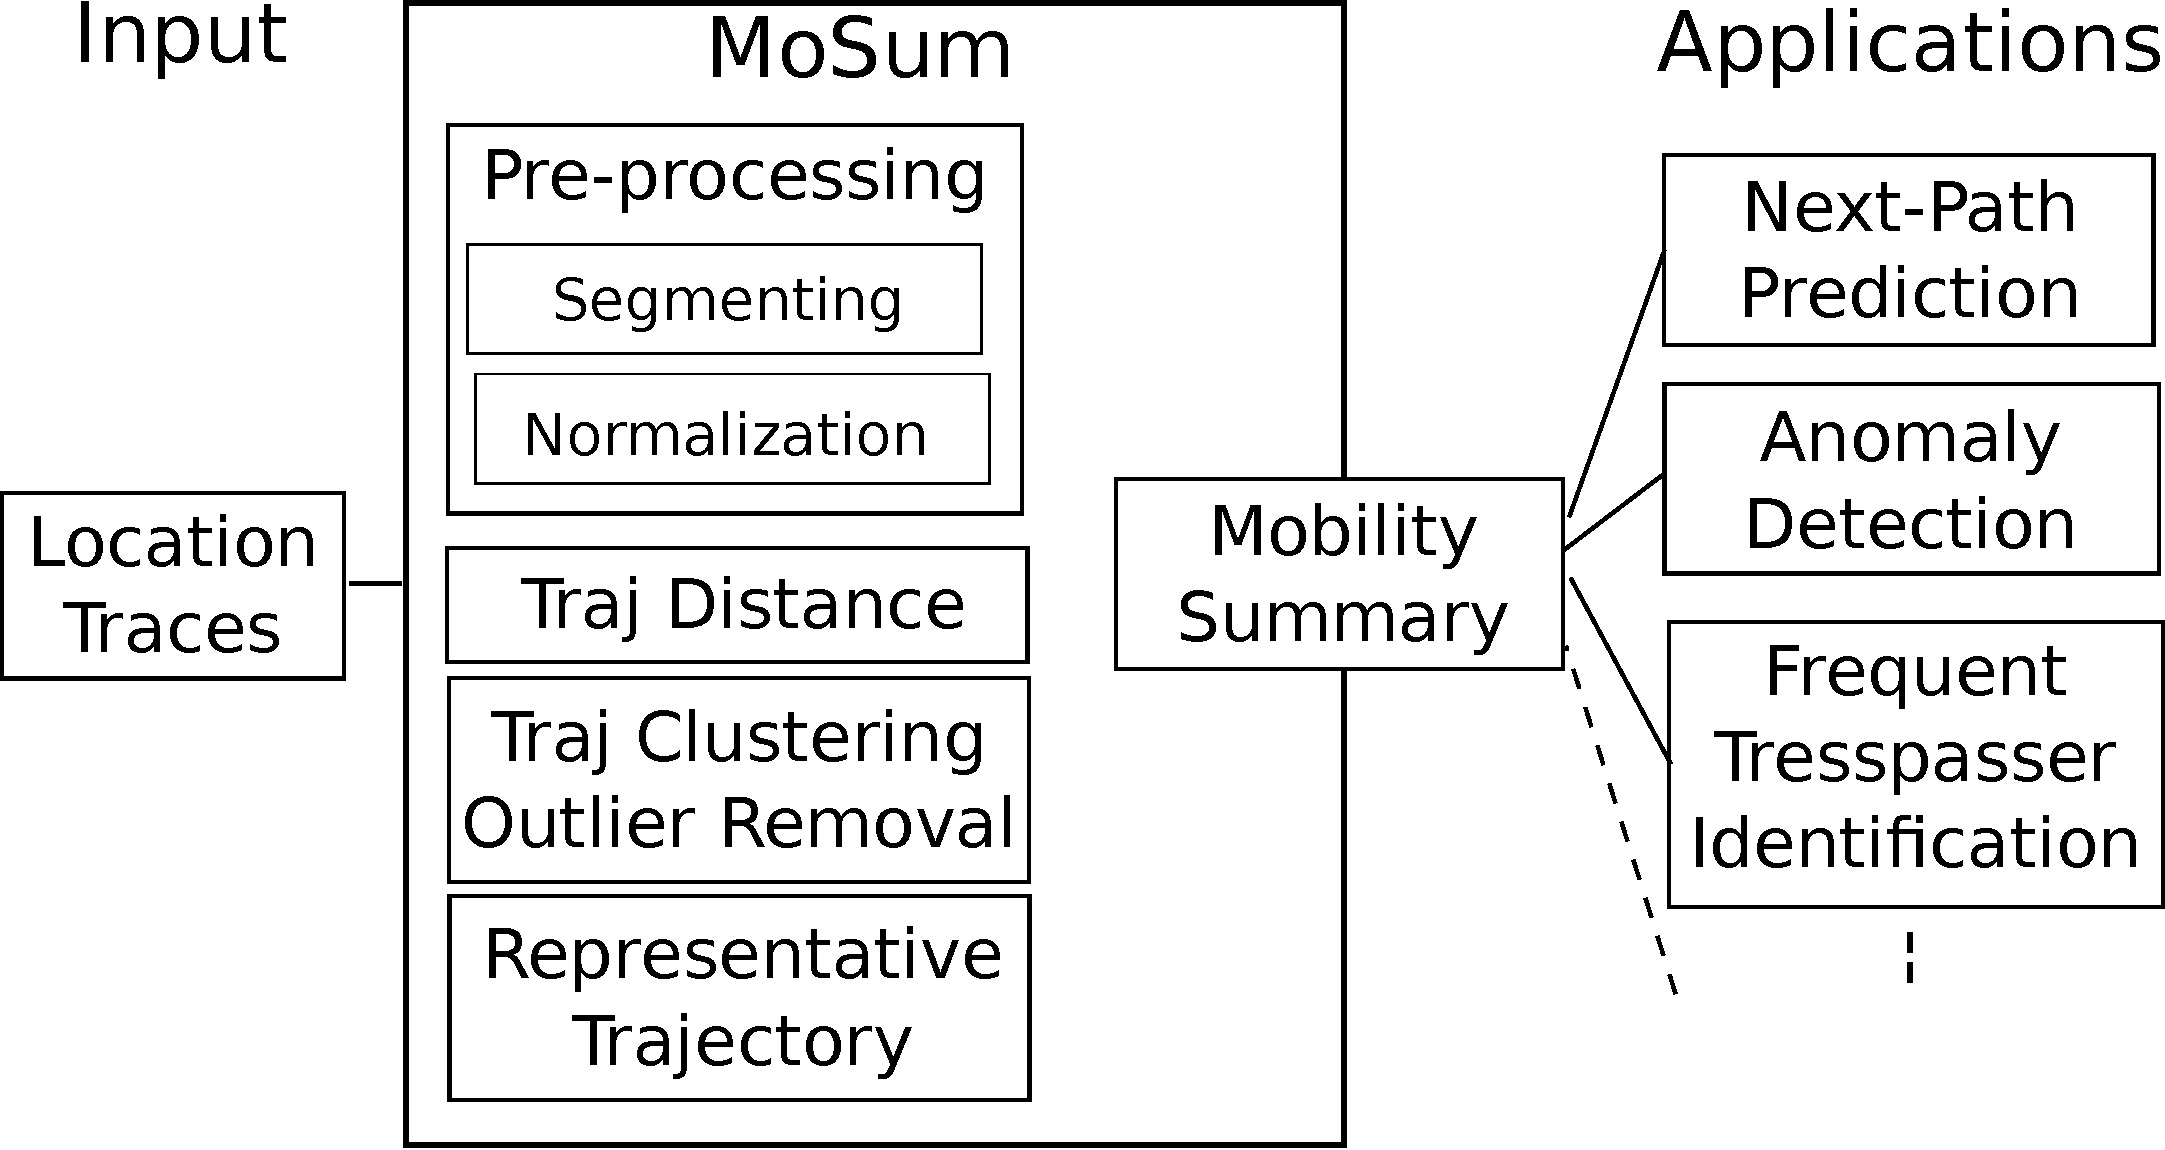
\includegraphics[width=7cm]{figs/overview.pdf}
\caption{MoSum Components}
\label{fig:components}
\end{figure}

Figure 1 provides the different components for computing the Mobility Summary, which in turn can be used a variety of applications that rely on frequent-mobility based queries. We now describe the components of MoSum in detail

%% 1 Trajectory Segmentation
%% 2. Trajectory Similarity
%% 3. Clustering
%% 

We first identify meaningful trips of a user using trajectory segmentation approaches~\cite{Zheng2008}. Here we compute the distance, velocity and time-gap between consecutive set of sample points to identify if the user is mobile. We use the well-known representation of trajectory to denote a meaningful trip; it is an ordered set of 3-tuples $\langle \operatorname{latitude},\operatorname{longitude},\operatorname{time} \rangle$.

We next normalize the user locations since small changes in latitude and longitude can result in large distances on earth. We normalize each raw latitude $\rawlat_i$ in the sample into a normalized latitude $\lat_i$ in the range $[0,1]$ as:
\begin{eqnarray}
\lat_i =\frac{\rawlat_i - \minlat}{\maxlat - \minlat}
\end{eqnarray}
where $\minlat=\min(\rawlat_j, \forall j)$ is the minimum latitude observed, and $\maxlat=\max(\rawlat_j, \forall j)$. We similarly normalize raw longitude and time values into normalized longitude and time values.

\section{Inter-Trajectory Distance}
\begin{table*}
	\centering
		\begin{tabular}{|c|c|c|c|c|c|} 
			\hline
			Sim Measure&Is Metric&Type&Sen. to sample noise&OD Cognizant&Computational Cost\\
			\hline
			LP Norm&Yes&Sampling Sensitive&No&No&O(N)\\
			DTW/LCSS/EDW/EDW With real sequences&No&Sampling Sensitive&Yes&No&O($n^2$)\\
			EDWP&Yes&Sampling Sensitive&Yes&No&??\\
			LP Norm with Interpolation&Yes&Shape Sensitive&No&No&O(Num samples)\\
			ODSim (Ours)&Yes&Shape sensitive&No&No&O(Num samples)\\
			\hline
		\end{tabular}
	\caption{Taxonomy of Similarity Measures}
	\label{tab:simTaxonomy}
\end{table*}
Computing the distance between a pair of trajectories is crucial to MoSum because of higher level clustering algorithms require such a distance measure. A large number of trajectory similarity metrics, which give an estimate of the trajectory distance, have been proposed for various types of applications. Standard LP-Norm and ERP have been shown to be metrics~\cite{Chen2004}, where as a large number of other heuristic measures (such as LCSS, DTW, EDR) are non-metrics~\cite{Vlachos2002,Yi1998,Chen2005}. A taxonomy of trajectory similarity metrics is discussed in Table~\ref{tab:simTaxonomy}. 

Non-metric distance functions are clearly inappropriate in clustering. In addition, we show that blindly using the existing non-metric distance functions not only results in sub-optimal clusters but also incurs significant high cost in terms of computational time. A primary reason for the most non-metric functions (LCSS, DTW, EDR, ERP) are designed to suppress noise using techniques such as dynamic programming. However, for GPS trajectory, de-noising can be done as a preprocessing step by removing or resampling the outlier points~\cite{Yuan2013,Zheng2009}. Hence, we use modified standard LP-Norm functions for distance computation, and avoid time consuming non-metric algorithms.

\subsection{Curve Distance for Trajectories}
Instead of treating trajectory as a set of sample points, we approximate the trajectories as curves on n-dimensional vector space. This approximation is reasonable if the location traces contains finely sampled GPS points (as in our case)\rednote{Need more justification and some defense here. Basically, if not LP-Norm will work too}. 

\rednote{Vinay: Karthik, please improve the below gibberish. I have taken the representation from Sebastien's paper}
For trajectory representation, the main idea is to represent trajectory as a curve in two independent dimensions latitude and longitude (in $\mathbb{R}^2$)~\cite{Kurtek2012}. A natural extension is to represent in three independent dimensions including time. However, in this paper, we propose to look at latitude and longitude dimensions \rednote{Why are we ignoring time? We dont know how to weigh time and space together while measuring distances}. 

Let $f_i:[0,1] \rightarrow \mathbb{R}^2$ be the curve for the $\operatorname{i}$-th trajectory trajectory, which maps a number between 0 to 1 to the (latitude, longitude) pairs of the trajectory. The standard $\mathbb{L}^2$ norm for this curve is given $\norm{f_i} = \left[ \int_{0}^{1}{f_i(x)^2\, \mathrm{d}x }\right] ^ {\frac{1}{2}}$. \rednote{Karthik: Please correct this. How does the next sentence fall out from the prev definitions?} With this notion, the Curve Distance (CD) between two trajectories $t_i$ and $t_j$ is given by the $\mathbb{L}^2$ distance:
\begin{align}
\LP(t_i,t_j) = \left[ \int_{0}^{1}{\left(f_i(x) - f_j(x) \right )^2\, \mathrm{d}x }\right] ^ {\frac{1}{2}}.
\end{align}

Numerically, we solve this by first resampling the trajectory at a large number of points for each trajectory (100 samples in our case) and then using Trapezoidal Rule~\cite{trapez} to find the curve distance. \rednote{Vinay: Karthik, Can you fill a good refernce for trapezoidal rule}.

\paragraph{Weighted Curve Distance} For human mobility, a user's meaningful trip has an associated intention (such as commuting to work or grocery shop visit). More often, each frequent trajectory are between end-points that are important to the user (such as home and work). We now propose a metric that emphasizes origin and destination of the trajectories, while computing the distance. 

We first generalize the Curve Distance to Weighted Curve Distance, where all trajectories have different weights at each point.  It can be shown the Weighted Curve Distance (WCD) between two trajectories $t_i$ and $t_j$ is given by
\begin{align}
\weightLP(t_i,t_j) = \left[ \int_{0}^{1}{ w(x) \left( f_i(x) - f_j(x) \right )^2\, \mathrm{d}x }\right] ^ {\frac{1}{2}}.
\end{align}
\noindent where $w(x) \rightarrow [0,1]$ is a weighting function. In the case of providing higher weights to origin and destination an Origin-Destination (OD) weighing function should be constructed such that the weights are high at the ends than at the center. We use Beta function $\operatorname{B(\alpha,\alpha)}$, where $\alpha$ in $[0,1]$. This provides a bimodal curve where weights at the ends are higher than the weights at the intermediate points in th curve; lower values of alpha provide very high values at ends than at the intermediate points.

Since CD is a metric and WCD is a weighted combination of CD (with positive weights), it can be shown that WCD is also a metric.\rednote{Vinay: Karthik, please comment}. 

\rednote{$===================$Karthik Checkpoint end$===================$}
\section{Trajectory Clustering}
We use the distance metrics to aggregate similar trajectories into one cluster. We use hierarchical agglomerative clustering since it provides the flexibility of analyzing the entire merge history of user's trajectories, and then cutting the dendogram at the right level. This enables us to personalize and automate clusters for different users. Each user has different motion patterns and -- apriori -- we do not have information of how often/densely a user travels along different paths. Our system automatically recognizes the right number of clusters by analyzing the dendogram.

We use ``average'' link clustering to measure similarity between intermediate clusters. This is to avoid bias for clustering trajectories that are associatively near (using single-link) or by concentrating on the extreme points of the merge (using complete-link).\rednote{Explain clearly. Show that complete or single has problems. Then say that DBSCAN also has problems. More probably so if single-link does not give good results}

\subsection{Finding optimal clusters}
In this step, we cut the dendogram at a level that defines meaningful mobility clusters. The main idea is to determine the optimal number of clusters for each person, and to use that knowledge to cut the dendogram. We went against determining a static similarity level to cut dendogram since different people have different forms of mobility. A user whose main travel pattern is long distance commute to two office locations has different distance thresholds than a student who is commuting mainly commuting from dormitory to classes. 

Existing well-known methods, such as the elbow method, do not cut the dendogram at appropriate level to provide good movement summaries; we demonstrate this in Section \label{sec:elbow}. Hence, we design an algorithm that cuts the dendogram at a level where trajectories in a cluster are between nearby origin and destinations, which signify similar meaningful trips of a person.
\rednote{Vinay: Manasa, can you please insert the algorithm (in latex algorithmic style)}

The algorithm iterates down the dendogram starting at the root; the number of clusters at this stage being $k=1$ . As we proceed down each level to cut the dendogram, the number of clusters $k$ increases by one. We compute the possible summary clusters of the user for each $k$. Let $\setSummClus_k =  \{ \summClus_{ki}, \forall i \}$ be the set of clusters for the user at level $k$. Let $t_{kij}$ be the $\operatorname{j}$-th trajectory in $\summClus_{kij}$. Let the mean trajectory for $\summClus_{ki}$ be $\meanTraj_{ki}$. We examine the tightness of clustering at this level by computing the Sum of Squares Within cluster (SSW). SSW at level $k$ is defined as $SSW_k=\sum_{\summClus_{ki} \in \setSummClus_k} \sum_{t_{kij} \in \summClus_{ki}} \weightLP(t_{kij},\meanTraj_{ki})^2$.

A well-known metric is to accept the elbow point of the $SSW_k$ vs. $k$ curve (say, at $k=k_e$) as the optimal number of clusters. However, as we show in Section~\ref{sec:elbowNotUseful}, the trajectories in clusters at the elbow point $k_e$ may contain multiple type of short trips in a small region; such trips can be split further into different cluster. Hence, we iterate from the elbow point towards greater $k$, and each $k$ we examine the resulting clusters to see if the trajectories from different types of meaningful trips are contained in a single cluster. We declare that different type of meaningful trips are present in a cluster if the physical distance between any point of any pair of trajectory curves in the cluster is greater than a intra-cluster separation distance $T_{\operatorname{intra}}$ (which is \unit{1.5}{km} in our case)\rednote{Vinay: Manasa, we need to figure this parameter out from the data set}. If distance is greater $T_{\operatorname{intra}}$, then we break this cluster further into multiple clusters by iterating down the dendogram. 

% Final summary
We finally represent the ``Mobility Summary'' of a user as the clusters with number of trajectories greater than a certain threshold (5\% of user's trajectories)\rednote{Vinay: Manasa, we need to figure this parameter out from the data set}. The rest of the trajectories are treated as anomalous trajectories. Each summary cluster and trajectories are represented similar definitions given above but we drop the subscript $k$, i.e. $\summClus=\{\summClus_i,\forall i\}$, $\summClus_i=\{t_{ij}, \forall j\}$, and $\meanTraj_i$ is the mean trajectory for cluster $i$. 

\begin{comment}
\subsection{Finding optimal clusters}
Number of clusters in the summary: Since each person's movement is unique(?), the number of clusters and the number of trajectories expected in each clusters are not constant. Hence, standard mechanisms such as k-means clustering cannot be directly applied to summarize. Even after the clusters are found out, we need to see if this cluster represents points that have meaningful end-to-end trips. \rednote{This is not coming out good. Need to think}
We need good OD +  we need trajectories that are not far away in the middle. One way to design a sim metric that is cognizant of: (1) origins, destinations, directionality and (2) the maximum separation between the trajectories. However, such a sim metric will introduce other artifacts (say, by classifying far away trajectories into same cluster). Hence we consider an approach where we decouple by considering O/D and direction in the sim metric, and then design an algorithm to select optimal number of clusters by looking at the maximum intra-cluster separation.
\end{comment}

\subsection{Representative trajectories}
We now find a representative trajectory for each of the cluster that can be used as a proxy for a summary cluster. One approach is to consider the mean trajectory curve $\meanTraj_i$ as a representative for the cluster $\summClus_i$. However, since the mean of multiple curves may not fall on any of the individual trajectories (and hence the roads on which the user went), it is not recommended as a representative. Hence, we follow a well-known method of computing piece-wise median trajectories~\cite{medianTraj}. Here, at an interval of $\delta$ number of points on interpolated mean trajectory, one point on any of the trajectories in the cluster closest to the mean is added to the representative trajectory. 

\begin{comment}
\subsection{Storing the trajectories at various levels of granularity}
\subsection{Intra-cluster Movement Pattern}
\end{comment}

\begin{comment}
Similarity metric for summarizing human movement should consider the below aspects
\begin{itemize}
\item Importance to Origins and Destinations: Hurricanes and other physical effects (?) are generally governed by physical laws and computing similarity might have to account for different effects. However, movement of a people is generally associated with an intention (such as commuting to work) of moving from an origin point to a destination point. Hence, a reasonable summary of a person's movement accounts for end-to-end trips that she takes. Currently, there is no similarity metric that gives any bias to the endpoints of the trajectory. We try to plug the bias into our similarity metric so that trip intentions are also given importance. 
For example, SWARM does not consider explicitly consider the end points of the trajectory. Hence, it might wrongly categorize movement on similar roads -- even with varying end points -- into the same cluster. \rednote{Show a toy scenario that shows how SWARM has mistook two different o-d clusters to be in the same cluster}

\item Metric: Clustering trajectories using standard clustering algorithms require the distance function between two trajectories to be a mathematical metric. In the current literature, only a few functions are metrics \cite{lp,edwp}. Others, which mostly take care of artifacts of sampling, are shown to be non-metrics. Using such functions, which violate properties like triangular inequality, in clustering can lead to unforeseen results. \rednote{Show a figure where tri inequality is violated in actual sense}
Ex of triangle inequality - User 014 ; Trajs 3,11,175;
3-175(124)>3-11(94)+11-175(4.283)

\item Sampling artifacts: Is time stretching and shrinking important? Are sampling points important? Ours is better because we consider human specific movement where direction and OD are important. While sampling frequency and alignment of samples is required, more or less all traces can be preprocessed after good samples have been taken. So, it really doesnt make sense to consider the effect of timing of samples (like DTW) while designing the clustering algorithm. \rednote{Vinay: Show a toy scenario where DTW goes wrong}
\end{itemize}

\paragraph{Origin-Destination}
In human movement, similar trips are usually between similar origin and destination regions. For example, the summary of a vast majority of working population are their trajectories between home and office. Hence, the similarity function should provide greater importance to OD. We define \textit{Weighted LP-Norm for OD} as
\begin{align}
w_{\od}(t, c, r) &= 
	\begin{cases} 
		\frac{c}{r} &\mbox{if } t \le \frac{r}{2} \mbox{ or } t > (1 - \frac{r}{2}), \\ 
		\frac{1- \frac{c}{r}}{(1-r)} & \mbox{otherwise},
	\end{cases}
\end{align}
\noindent where $r$ and $c$ denote the parameters define the weight assigned to the origin and destination stertches when compared to the intermediate stretch. Here $r$ defines the fraction of the stretch from origin or towards destination which has to be given a prominence ($r=[0,1]$). And, $c$ is the weight assignment factor at O and D stretches ($c=[0,1]$). If $c > 1 -r$, then the origin and destination stretches of length $\frac{r}{2}$, will be given a higher weight than the intermediate stretch (of length $1 - r$)


\noindent
For Uma's work:
Let $x_i \ge 0$ represent the ``color of grid $i$''. \\
Let $N(i) = \left \{ \text{All grids that are neighbors of i} \right \}$. \\
Let $C$ be the ``conflicting set''. A tuple $(i,j)$ is added to the conflicting set $C$ if two grids $i$ and $j$ have a \textit{LAC separating line} between them.\\
Let $y_i$ be an indicator variable to say if the grid has same color as atleast one of its neighbor.

We formulate an optimization problem to find the color for each grid as below:
\begin{align}
\mbox{Min} \sum_{i}{y_i}
\end{align}
\noindent such that:
\begin{align}
x_i &\neq x_j, ~~~\forall (i,j) \in C\\
y_i &= 
\begin{cases} 
		1 &\mbox{if } \forall j=N(i), x_i = x_j, \\ 
		0 &\mbox{otherwise}.
	\end{cases}
\end{align}

In order to assign similarity scores  to pairs of trajectories, we first have to resample them into equal number of points. 
\paragraph{Resampling and Interpolation}
\paragraph{Using Linear Interpolation over Spline}
\rednote Image showing problems when using spline interpolation 
\begin{figure}
\centering
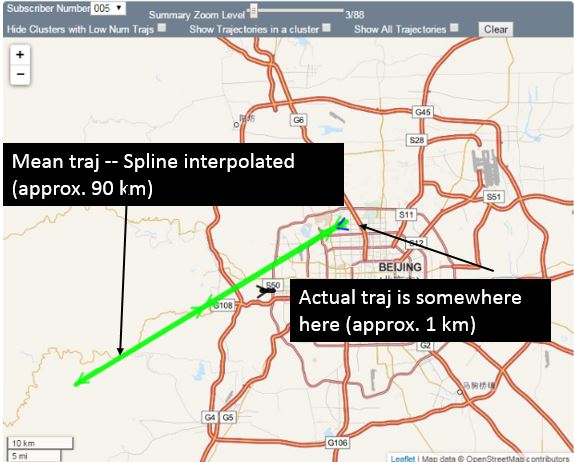
\includegraphics[scale=0.4]{figs/spline.jpg}
\caption{Problems with spline interpolation}
\label{fig:spline}
\end{figure}
\paragraph{Resampling and then applying DTW is very close to using our similarity measure }
\end{comment}
\section{Work Done}
\subsection{Trajectory Preprocesing} 

\paragraph{Segmentation}
The first step in pre-processing is to identify meaningful trips of a user using trajectory segmentation approaches~\cite{Zheng2008}. The input to the module is a raw file of three tuples containing the latitude and longitude of the user sampled at various time instances. This does not necessarily consist of moving trajectories, it might also contain tuples where the user is static for a long time. The aim is to eliminate such tuples, and extract only the meaningful trajectories where the user is in motion or has made a trip. Here the distance, velocity and time-gap between consecutive set of sample points are computed to identify if the user is mobile. The well-known representation of trajectory to denote a meaningful trip is used; it is an ordered set of 3-tuples $\langle \operatorname{latitude},\operatorname{longitude},\operatorname{time} \rangle$.
\paragraph{Normalization}
The next step is to normalize the user locations since small changes in latitude and longitude can result in large distances on earth. Each raw latitude $\rawlat_i$ in the sample is normalized into a normalized latitude $\lat_i$ in the range $[0,1]$ as:
\begin{eqnarray}
\lat_i =\frac{\rawlat_i - \minlat}{\maxlat - \minlat}
\end{eqnarray}
where $\minlat=\min(\rawlat_j, \forall j)$ is the minimum latitude observed, and $\maxlat=\max(\rawlat_j, \forall j)$. 

Similarly, the raw longitude $\rawlon_i$ in converted to a normalized longitude $\lon_i$ in the range $[0,1]$ as:
\begin{eqnarray}
\lon_i =\frac{\rawlon_i - \minlon}{\maxlon - \minlon}
\end{eqnarray}
where $\minlon=\min(\rawlon_j, \forall j)$ is the minimum longitude observed, and $\maxlon=\max(\rawlon_j, \forall j)$. 


\subsection{Trajectory Similarity}

Computing the distance between a pair of trajectories is crucial to \trajSummary because of higher level clustering algorithms require such a distance measure. A large number of trajectory similarity metrics, which give an estimate of the trajectory distance, have been proposed for various types of applications. Standard LP-Norm and ERP have been shown to be metrics~\cite{Chen2004}, where as a large number of other heuristic measures (such as LCSS, DTW, EDR) are non-metrics~\cite{Vlachos2002,Yi1998,Chen2005}. A taxonomy of trajectory similarity metrics is discussed in Table~\ref{tab:simTaxonomy}. 
\begin{table*}
	\centering
	\resizebox{\textwidth}{!}{
		\begin{tabular}{|c|c|c|c|c|c|} 
			\hline
			Sim Measure&Is Metric&Type&Sen. to sample noise&OD Cognizant&Computational Cost\\
			\hline
			LP Norm&Yes&Sampling Sensitive&No&No&O(N)\\
			DTW/LCSS/EDW/EDW With real sequences&No&Sampling Sensitive&Yes&No&O($n^2$)\\
%			EDWP&Yes&Sampling Sensitive&Yes&No&??\\
			LP Norm with Interpolation&Yes&Shape Sensitive&No&No&O(Num samples)\\
			ODSim (Ours)&Yes&Shape sensitive&No&No&O(Num samples)\\
			\hline
		\end{tabular}}
	\caption{Taxonomy of Similarity Measures}
	\label{tab:simTaxonomy}
\end{table*}

The table talks about various features of a similarity function described as follows:\\
Is Metric:It is important for a similarity measure to be mathematical metric. The conditions for being a mathematical metric are it should be symmetric, values should be non-negative, and it should follow triangle inequality. If a similarity measure is not a metric, problems might come up while clustering based on the similarity matrix. \\
Type: Sampling sensitive measures vary hugely on the way the data points are sampled and the time interval at which they are sampled. Shape sensitive measures give more importance to the shape of the trajectory than the sample points, thus making it more robust.\\
Sensitive to sampling noise\\
Origin-Destination Cognizant : As the mobility summary is defined for human movement, it would be an advantage if the similarity measure is Origin-Destination cognizant.\\
Computation Cost.\\

Non-metric distance functions are clearly inappropriate in clustering. In addition, we show that blindly using the existing non-metric distance functions not only results in sub-optimal clusters but also incurs significant high cost in terms of computational time. A primary reason for the most non-metric functions (LCSS, DTW, EDR, ERP) are designed to suppress noise using techniques such as dynamic programming. However, for GPS trajectory, de-noising can be done as a preprocessing step by removing or resampling the outlier points~\cite{Yuan2013,Zheng2009}. Hence, the modified standard LP-Norm functions are used for distance computation, and avoid time consuming non-metric algorithms.

\subsubsection{Curve Distance for Trajectories}
Instead of treating trajectory as a set of sample points, the trajectories can be approximated as curves on n-dimensional vector space. This approximation is reasonable if the location traces contain finely sampled GPS points (as in this case)%\rednote{Need more justification and some defense here. Basically, if not LP-Norm will work too}. 

%\rednote{Vinay: Karthik, please improve the below gibberish. I have taken the representation from Sebastien's paper}
For trajectory representation, the main idea is to represent trajectory as a curve in two independent dimensions latitude and longitude (in $\mathbb{R}^2$)~\cite{Kurtek2012}. A natural extension is to represent in three independent dimensions including time. However, in this work, only latitude and longitude dimensions are looked into. %\rednote{Why are we ignoring time? We dont know how to weigh time and space together while measuring distances}. 

Let $f_i[0,1] \rightarrow \mathbb{R}^2$ be the curve for the $\operatorname{i}$-th trajectory trajectory, which maps a number between 0 to 1 to the (latitude, longitude) pairs of the trajectory. The standard $\mathbb{L}^2$ norm for this curve is given $\norm{f_i} = \left[ \int_{0}^{1}{f_i(x)^2\, \mathrm{d}x }\right] ^ {\frac{1}{2}}$. %\rednote{Karthik: Please correct this. How does the next sentence fall out from the prev definitions?} With this notion, the Curve Distance (CD) between two trajectories $t_i$ and $t_j$ is given by the $\mathbb{L}^2$ distance:
\begin{align}
\LP(t_i,t_j) = \left[ \int_{0}^{1}{\left(f_i(x) - f_j(x) \right )^2\, \mathrm{d}x }\right] ^ {\frac{1}{2}}.
\end{align}

Numerically, this is solved by first resampling the trajectory to a large number of points for each trajectory (100 samples in our case) and then using Trapezoidal Rule to find the curve distance. %\rednote{Vinay: Karthik, Can you fill a good refernce for trapezoidal rule}.

\paragraph{Weighted Curve Distance} For human mobility, a user's meaningful trip has an associated intention (such as commuting to work or grocery shop visit). More often, each frequent trajectory are between end-points that are important to the user (such as home and work). A metric is hence proposed that emphasizes origin and destination of the trajectories, while computing the distance. 

We first generalize the Curve Distance to Weighted Curve Distance, where all trajectories have different weights at each point.  It can be shown the Weighted Curve Distance (WCD) between two trajectories $t_i$ and $t_j$ is given by
\begin{align}
\weightLP(t_i,t_j) = \left[ \int_{0}^{1}{ w(x) \left( f_i(x) - f_j(x) \right )^2\, \mathrm{d}x }\right] ^ {\frac{1}{2}}.
\end{align}
\noindent where $w(x) \rightarrow [0,1]$ is a weighting function. In the case of providing higher weights to origin and destination an Origin-Destination (OD) weighing function should be constructed such that the weights are high at the ends than at the center. We use Beta function $\operatorname{B(\alpha,\alpha)}$, where $\alpha$ in $[0,1]$. This provides a bimodal curve where weights at the ends are higher than the weights at the intermediate points in th curve; lower values of alpha provide very high values at ends than at the intermediate points.

Since CD is a metric and WCD is a weighted combination of CD (with positive weights), it can be shown that WCD is also a metric.

%\rednote{Vinay: Karthik, please comment}. 

%
%\begin{comment}
%%\rednote{$===================$Karthik Checkpoint end$===================$}
%\section{Trajectory Clustering}
%We use the distance metrics to aggregate similar trajectories into one cluster. We use hierarchical agglomerative clustering since it provides the flexibility of analyzing the entire merge history of user's trajectories, and then cutting the dendrogram at the right level. This enables us to personalize and automate clusters for different users. Each user has different motion patterns and -- apriori -- we do not have information of how often/densely a user travels along different paths. Our system automatically recognizes the right number of clusters by analyzing the dendrogram.
%
%We use ``average'' link clustering to measure similarity between intermediate clusters. This is to avoid bias for clustering trajectories that are associatively near (using single-link) or by concentrating on the extreme points of the merge (using complete-link).%\rednote{Explain clearly. Show that complete or single has problems. Then say that DBSCAN also has problems. More probably so if single-link does not give good results}
%
%\subsection{Finding optimal clusters}
%In this step, we cut the dendrogram at a level that defines meaningful mobility clusters. The main idea is to determine the optimal number of clusters for each person, and to use that knowledge to cut the dendrogram. We went against determining a static similarity level to cut dendrogram since different people have different forms of mobility. A user whose main travel pattern is long distance commute to two office locations has different distance thresholds than a student who is commuting mainly commuting from dormitory to classes. 
%
%Existing well-known methods, such as the elbow method, do not cut the dendogram at appropriate level to provide good movement summaries; we demonstrate this in Section \label{sec:elbow}. Hence, we design an algorithm that cuts the dendogram at a level where trajectories in a cluster are between nearby origin and destinations, which signify similar meaningful trips of a person.
%\newenvironment{badidea}
%  {\par\leftskip=2cm}
%  {\par}
%\begin{algorithm}
%\KwIn{Dendrogram with cluster information at each level}
%\KwOut{Optimal Clusters (Trip Summaries)}    
%
%\SetAlgoLined
%\SetKwFunction{isSummary}{isSummary}
%\For{\text{k=1 to N}}
%{
%\begin{equation}
%SSW(Clus_i)= \sum_{j=1}^{|Trajs(Clus_i)|}{Sim(Traj_{j},Mean(Clus_i))}
%\end{equation}
%\begin{equation}
%SSW(Level_k)=\sum_{j=1}^{k}{SSW(Cluster_j)}
%\end{equation}
%}
%Find the elbow point from the SSW Plot over all levels \\
%Set all trajectories as \textit{unmarked}
%\For{\text{k=elbowPoint+1 to N}}
%{
%\For{\text{Each non anomalous  cluster}}
%{
%\If{Trajs(Cluster) are unmarked \&\& \isSummary{$Cluster_i$} }
%{
%Report Cluster as a final Cluster\\
%Mark all Trajs in Cluster
%}
%}
%}
%\isSummary{$Cluster_i$}{
%
%\For{All pairs of trajectories in Cluster}
%{
% \If{Maximum Pointwise Distance$\le$ $\delta$  (kms)}
% {
%\KwRet True}
%}
%\KwRet False
%}
%\\
%
%\caption{Algorithm for reporting final clusters from Dendrogram}
%
%\end{algorithm}
%
%%\rednote{Vinay: Manasa, can you please insert the algorithm (in latex algorithmic style)}
%
%The algorithm iterates down the dendrogram starting at the root; the number of clusters at this stage being $k=1$ . As we proceed down each level to cut the dendrogram, the number of clusters $k$ increases by one. We compute the possible summary clusters of the user for each $k$. Let $\setSummClus_k =  \{ \summClus_{ki}, \forall i \}$ be the set of clusters for the user at level $k$. Let $t_{kij}$ be the $\operatorname{j}$-th trajectory in $\summClus_{kij}$. Let the mean trajectory for $\summClus_{ki}$ be $\meanTraj_{ki}$. We examine the tightness of clustering at this level by computing the Sum of Squares Within cluster (SSW). SSW at level $k$ is defined as $SSW_k=\sum_{\summClus_{ki} \in \setSummClus_k} \sum_{t_{kij} \in \summClus_{ki}} \weightLP(t_{kij},\meanTraj_{ki})^2$.
%
%A well-known metric is to accept the elbow point of the $SSW_k$ vs. $k$ curve (say, at $k=k_e$) as the optimal number of clusters. However, as we show in Section 7, the trajectories in clusters at the elbow point $k_e$ may contain multiple type of short trips in a small region; such trips can be split further into different cluster. Hence, we iterate from the elbow point towards greater $k$, and each $k$ we examine the resulting clusters to see if the trajectories from different types of meaningful trips are contained in a single cluster. We declare that different type of meaningful trips are present in a cluster if the physical distance between any point of any pair of trajectory curves in the cluster is greater than a intra-cluster separation distance $T_{\operatorname{intra}}$ (which is \unit{1.5}{km} in our case)%\rednote{Vinay: Manasa, we need to figure this parameter out from the data set}. If distance is greater $T_{\operatorname{intra}}$, then we break this cluster further into multiple clusters by iterating down the dendogram. 
%
%% Final summary
%We finally represent the ``Mobility Summary'' of a user as the clusters with number of trajectories greater than a certain threshold (5\% of user's trajectories)%\rednote{Vinay: Manasa, we need to figure this parameter out from the data set}. The rest of the trajectories are treated as anomalous trajectories. Each summary cluster and trajectories are represented similar definitions given above but we drop the subscript $k$, i.e. $\summClus=\{\summClus_i,\forall i\}$, $\summClus_i=\{t_{ij}, \forall j\}$, and $\meanTraj_i$ is the mean trajectory for cluster $i$. 
%
%
%\subsection{Finding optimal clusters}
%Number of clusters in the summary: Since each person's movement is unique(?), the number of clusters and the number of trajectories expected in each clusters are not constant. Hence, standard mechanisms such as k-means clustering cannot be directly applied to summarize. Even after the clusters are found out, we need to see if this cluster represents points that have meaningful end-to-end trips.% \rednote{This is not coming out good. Need to think}
%We need good OD +  we need trajectories that are not far away in the middle. One way to design a sim metric that is cognizant of: (1) origins, destinations, directionality and (2) the maximum separation between the trajectories. However, such a sim metric will introduce other artifacts (say, by classifying far away trajectories into same cluster). Hence we consider an approach where we decouple by considering O/D and direction in the sim metric, and then design an algorithm to select optimal number of clusters by looking at the maximum intra-cluster separation.
%
%
%\subsection{Representative trajectories}
%We now find a representative trajectory for each of the cluster that can be used as a proxy for a summary cluster. One approach is to consider the mean trajectory curve $\meanTraj_i$ as a representative for the cluster $\summClus_i$. However, since the mean of multiple curves may not fall on any of the individual trajectories (and hence the roads on which the user went), it is not recommended as a representative. Hence, we follow a well-known method of computing piece-wise median trajectories~\cite{median1}. Here, at an interval of $\delta$ number of points on interpolated mean trajectory, one point on any of the trajectories in the cluster closest to the mean is added to the representative trajectory. 
%\end{comment}
%\begin{comment}
%\subsection{Storing the trajectories at various levels of granularity}
%\subsection{Intra-cluster Movement Pattern}
%\end{comment}
%
%\begin{comment}
%Similarity metric for summarizing human movement should consider the below aspects
%\begin{itemize}
%\item Importance to Origins and Destinations: Hurricanes and other physical effects (?) are generally governed by physical laws and computing similarity might have to account for different effects. However, movement of a people is generally associated with an intention (such as commuting to work) of moving from an origin point to a destination point. Hence, a reasonable summary of a person's movement accounts for end-to-end trips that she takes. Currently, there is no similarity metric that gives any bias to the endpoints of the trajectory. We try to plug the bias into our similarity metric so that trip intentions are also given importance. 
%For example, SWARM does not consider explicitly consider the end points of the trajectory. Hence, it might wrongly categorize movement on similar roads -- even with varying end points -- into the same cluster. %\rednote{Show a toy scenario that shows how SWARM has mistook two different o-d clusters to be in the same cluster}
%
%\item Metric: Clustering trajectories using standard clustering algorithms require the distance function between two trajectories to be a mathematical metric. In the current literature, only a few functions are metrics \cite{lp,edwp}. Others, which mostly take care of artifacts of sampling, are shown to be non-metrics. Using such functions, which violate properties like triangular inequality, in clustering can lead to unforeseen results. %\rednote{Show a figure where tri inequality is violated in actual sense}
%Ex of triangle inequality - User 014 ; Trajs 3,11,175;
%3-175(124)>3-11(94)+11-175(4.283)
%
%\item Sampling artifacts: Is time stretching and shrinking important? Are sampling points important? Ours is better because we consider human specific movement where direction and OD are important. While sampling frequency and alignment of samples is required, more or less all traces can be preprocessed after good samples have been taken. So, it really doesnt make sense to consider the effect of timing of samples (like DTW) while designing the clustering algorithm. %\rednote{Vinay: Show a toy scenario where DTW goes wrong}
%\end{itemize}
%
%\paragraph{Origin-Destination}
%In human movement, similar trips are usually between similar origin and destination regions. For example, the summary of a vast majority of working population are their trajectories between home and office. Hence, the similarity function should provide greater importance to OD. We define \textit{Weighted LP-Norm for OD} as
%\begin{align}
%w_{\od}(t, c, r) &= 
%	\begin{cases} 
%		\frac{c}{r} &\mbox{if } t \le \frac{r}{2} \mbox{ or } t > (1 - \frac{r}{2}), \\ 
%		\frac{1- \frac{c}{r}}{(1-r)} & \mbox{otherwise},
%	\end{cases}
%\end{align}
%\noindent where $r$ and $c$ denote the parameters define the weight assigned to the origin and destination stertches when compared to the intermediate stretch. Here $r$ defines the fraction of the stretch from origin or towards destination which has to be given a prominence ($r=[0,1]$). And, $c$ is the weight assignment factor at O and D stretches ($c=[0,1]$). If $c > 1 -r$, then the origin and destination stretches of length $\frac{r}{2}$, will be given a higher weight than the intermediate stretch (of length $1 - r$)
%
%
%
%In order to assign similarity scores  to pairs of trajectories, we first have to resample them into equal number of points. 
%\paragraph{Resampling and Interpolation}
%\paragraph{Using Linear Interpolation over Spline}
%%\rednote Image showing problems when using spline interpolation 
%\begin{figure}
%\centering
%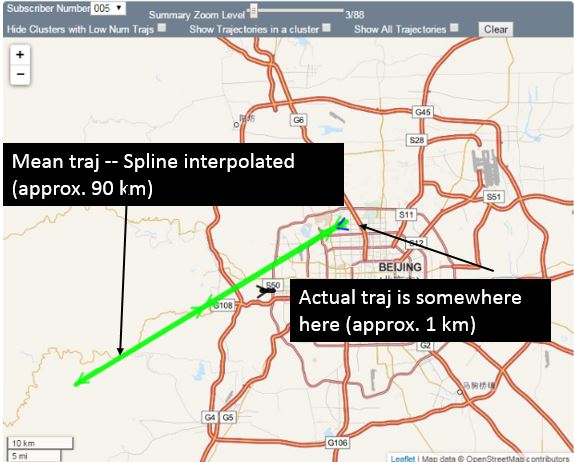
\includegraphics[scale=0.4]{figs/spline.jpg}
%\caption{Problems with spline interpolation}
%\label{fig:spline}
%\end{figure}
%\paragraph{Resampling and then applying DTW is very close to using our similarity measure }
%\end{comment}

\section{Evaluation and Analysis}

\subsection{Dataset}
\begin{itemize}
\item Microsoft GeoLife Dataset
GeoLife Dataset published by Microsoft Research \cite{geolife1},\cite{geolife2},\cite{geolife3}. This is a GPS trajectory dataset with GPS traces of 182 users over a period of three years (from April 2007 to August 2012). 
\item Microsoft T Drive Taxicab Dataset
This is a trajectory dataset that contains one-week trajectories of 10,357 taxis published by Microsoft Research. \cite{tdrive1} ,\cite{tdrive2}
\end{itemize}
\subsection{Clustering Effectiveness}
We have shown various comparisons and result, but the main measure of clustering effectiveness that we use is the Silhouette Coefficient(SC). SC is a standard metric that shows the effectiveness of clustering. SC is based on the cohesion and the separation of clusters formed. The cohesion ( \textit{a(x)})  is defined as the average distance of x to all other vectors in the same cluster. 
The separation (\textit{b(x)}) is defined as the minimum of the average distances of x to the vectors in other clusters.
Further, the silhouette coefficient of a data point is defined as 
\begin{equation}
s(x)=\frac{b(x)-a(x)}{max(a(x),b(x))}
\end{equation}
The total silhouette coefficient of the dataset is the average over all the points given by
\begin{equation}
SC=\frac{1}{N}\sum_{i=1}^{N}s(x)
\end{equation}
\noindent Ideally, SC is between [-1,1], where values closer to 1 representing better formed clusters. 

\subsection{Individual Movement Summary}

In this section, we talk about the experiments made on the Microsoft GeoLife Dataset. These are GPS traces of around 182 users collected over a period of three years. From this data, we aim at finding the movement summary of the person which will give us insights into how that person moves and which patters appear repeatedly. In the first section we show the working of our proposed method with supporting visuals at every step explaining the rationale behind it. Further, we implemented and modified some other works from the literature to suit the problem and have discussed the results. A brief description of the methods we have compared with are given below.

\paragraph{Dynamic Time Warping}
This is a comparison made in the choice of the similarity metric that we use. We show the effects of using DTW in place of our similarity measure, keeping everything else in the algorithm exactly as it is.The DTW similarity between A and B is defined below 
\begin{equation}
D_{dtw}(A,B) =
\left\{
	\begin{array}{ll}
		0  & \mbox{if } \text{both A and B are empty} \\
		\infty & \mbox{if } \text{one of A or B is empty}\\
                \phi _d (head(A),head(B))+
                   \\min 
\left\{
	\begin{array}{ll}
		D_{dtw}(A,rest(B)), \leftarrow \text{\emph{Stretch A}}\\

		D_{dtw}(rest(A),B),\leftarrow \text{\emph{Stretch B}}\\
                D_{dtw}(rest(A),rest(B)) 
	\end{array}
\right.          \\otherwise
	\end{array}
\right.
\end{equation}

where $\phi_d(p1,p2)=L_2-dist(p1,p2)$ 
\paragraph{SWARM}
SWARM is a moving objects clustering algorithm proposed by Li \emph{et al.}\cite{Li2010}  In this algorithm they consider trajectories to be of the same cluster if they are together in similar clusters for a specific number of (not necessarily consecutive) timestamps. 
\paragraph{TRACLUS}
 TRACLUS is an algorithm proposed by Lee \emph{et al.} in \cite{Lee2007}. This algorithm partitions the trajectories, clusters the partitions and then comes up with a final representative cluster. 


\subsubsection{Proposed Method-OD}
In this section we show each stage of the proposed method and the corresponding visualizations at that stage for a test user. 
Fig. \ref{fig:alltrajs} shows all the trajectories of the user. We compute the similarity matrix using the similarity defined earlier  and run hierarchical clustering on it. 

\begin{figure}
\centering     
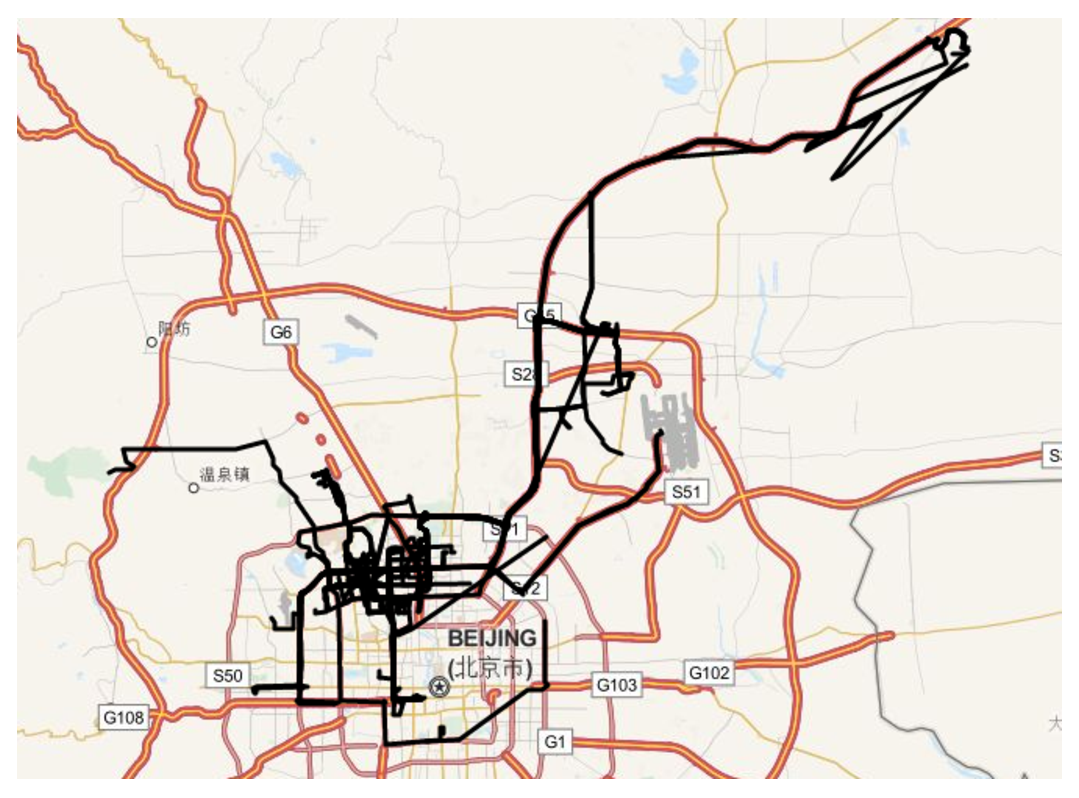
\includegraphics[scale=0.4]{figs/new/allTrajs.eps}
\caption{A snapshot of all the trajectories of the test user (363 trajectories in total)}
\label{fig:alltrajs}  
\end{figure}


The dendrogram is a pictoral representation of how similar the trajectories are among each other. The ones more similar to each other are paired closer to the bottom as compared to the ones higher in the tree. Fig \ref{fig:dendrogram} shows the dendrogram of the trajectories of the test user. The user had 363 trajectories in total, so the dendrogram has 363 leaves. 
\begin{figure}[t]
\centering     
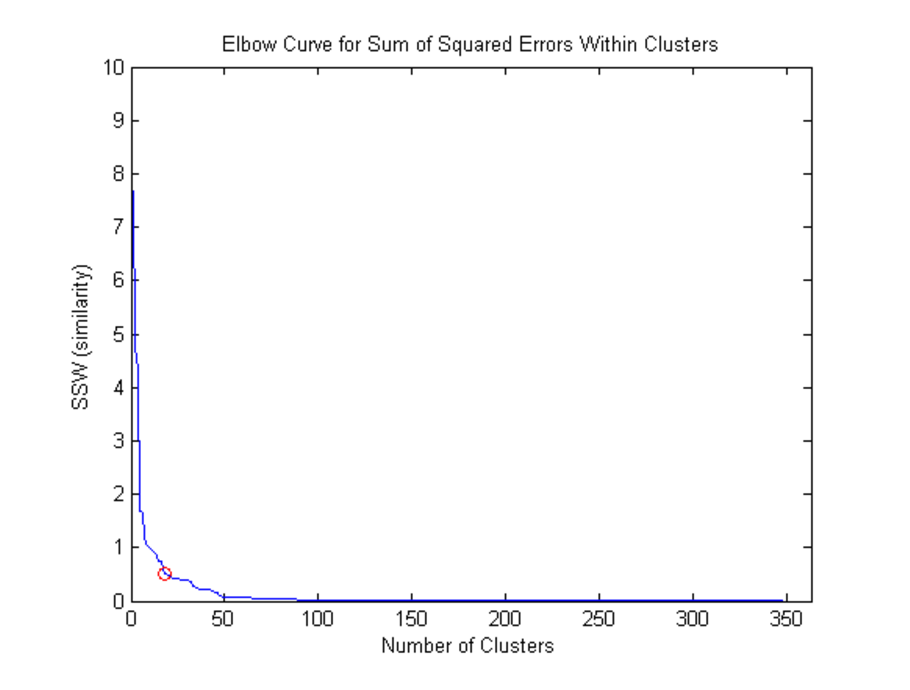
\includegraphics[scale=0.5]{figs/new/elbow.eps}
\caption{Elbow curve - Plot of the SSW vs number of Clusters; Elbow point ~ 18 clusters}
\label{fig:elbow}  
\end{figure}
\begin{figure*}
\centering     
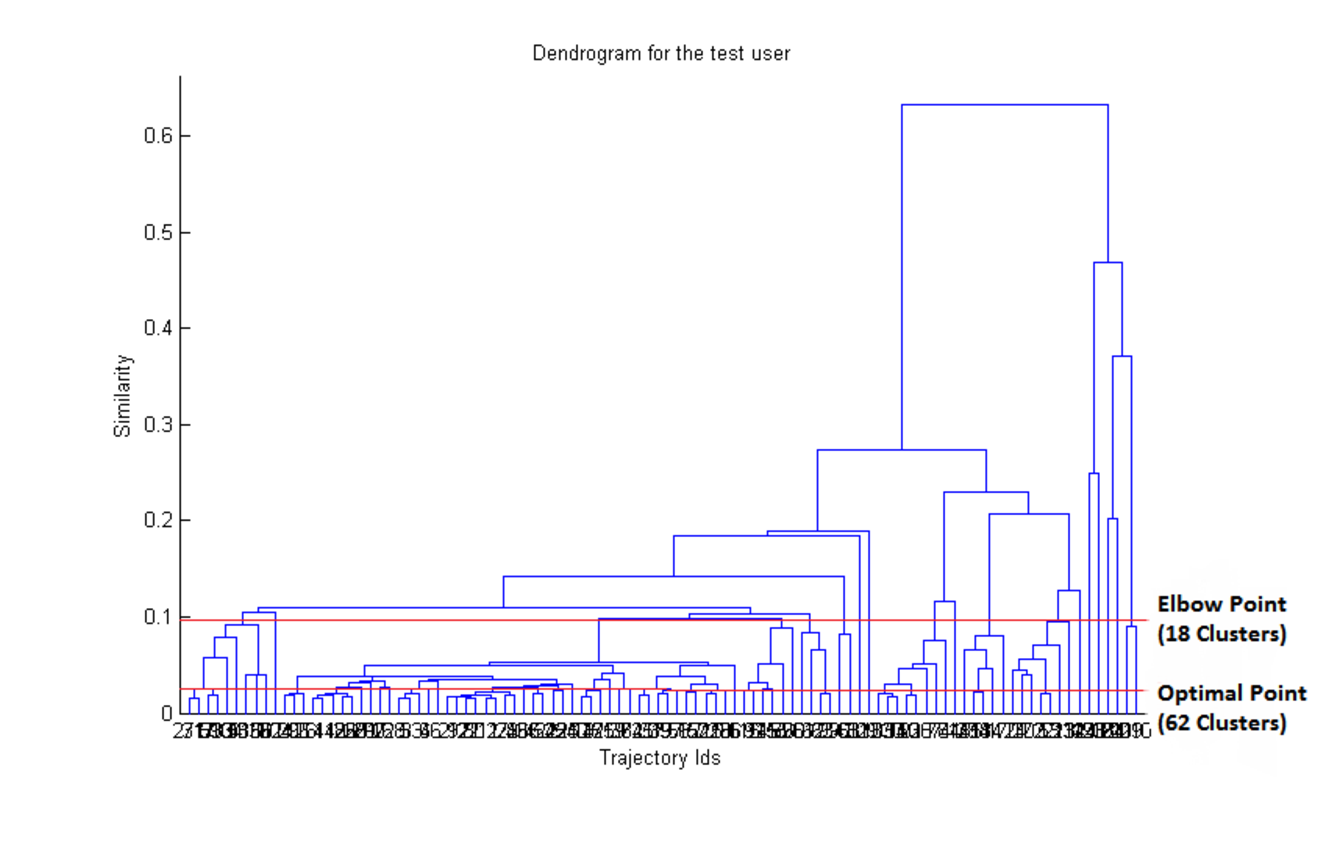
\includegraphics[scale=0.5]{figs/new/dendrogram.eps}
\caption{Dendrogram of the all the trajectories (Shows the hierarchy of similarity) The elbow point is at 18 clusters, whereas the optimal number of clusters is 62 }
\label{fig:dendrogram}  
\end{figure*}
To obtain a certain cluster of the trajectories, we have to cut the dendrogram at a certain level. The height at which we cut the dendrogram decides the number of clusters we will get. Finding the right height at which we should cut the dendrogram is one of the biggest challenges in coming up with an accurate summary for a user. One method which is widely used in literature is to plot the cumulative Sum of Squared Errors within Cluster as the cluster number varies from 1 to N. This is called the elbow curve or the scree plot and the elbow point in this curve should give us the right number of clusters. The rationale behind this is that we want to find the saturation point beyond which even on increasing the number of clusters, the error within the clusters doesnt decrease significantly. But, in our case, we found that the elbow point doesn't get us anywhere close to the actual optimal point of clustering. The validation of the clusters formed at each value of number of clusters was done by visualizing the results and looking at the general tightness of the clusters. Fig \ref{fig:elbow} shows the elbow curve with two lines indicating the elbow point, and the optimal cluster number. We see that the actual optimal point is way beyond the elbow point, and show the visualizations of the top 4 clusters at both the elbow point, in Fig. \ref{fig:elbowVisual} and (elbow point +5) number of clusters in Fig. \ref{fig:elbow5visual}.  


\begin{figure*}
    \centering
    \begin{subfigure}[t]{.5\textwidth}
        \centering
        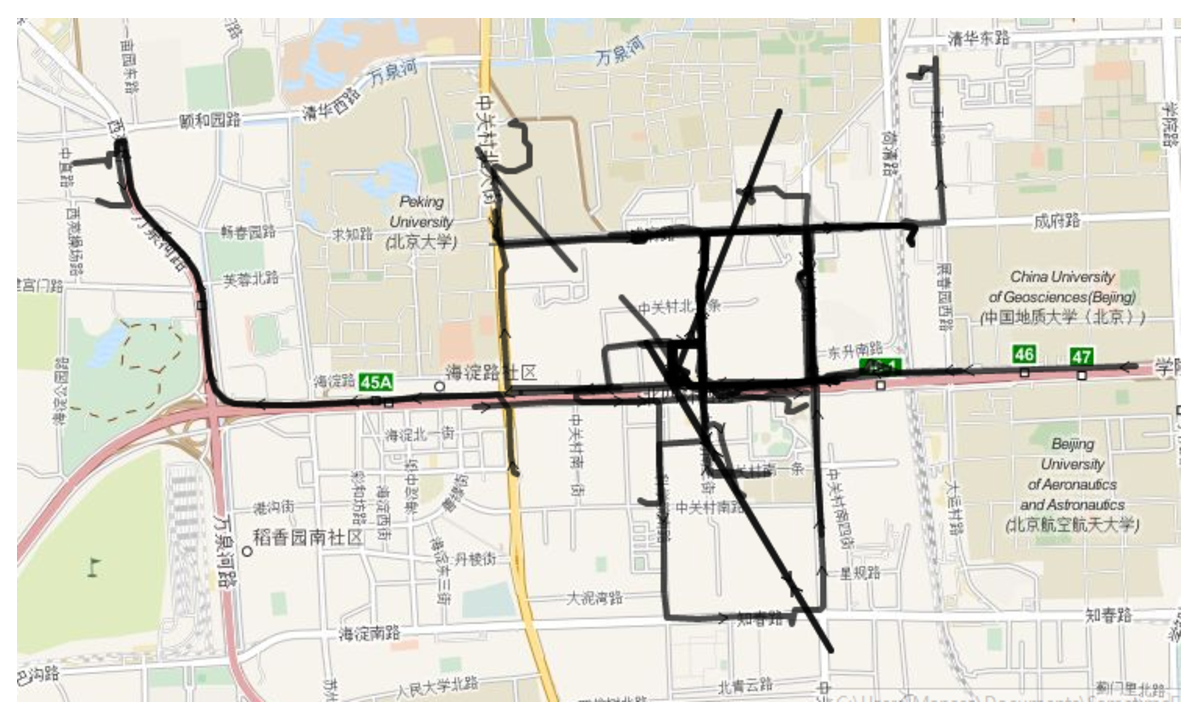
\includegraphics[width=6cm,height=4cm,keepaspectratio]{figs/new/Elbow_Cluster1.eps}
        \caption{Cluster 1 ( 32 trajectories)}
    \end{subfigure}%
    \begin{subfigure}[t]{.5\textwidth}
        \centering
        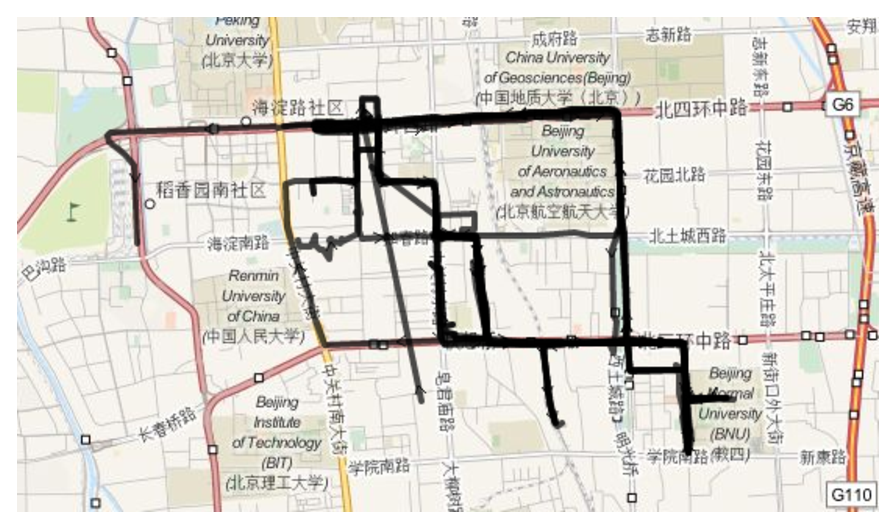
\includegraphics[width=6cm,height=4cm,keepaspectratio]{figs/new/Elbow_Cluster2.eps}
        \caption{Cluster 2(31 trajectories)}
    \end{subfigure}
        
    \begin{subfigure}[t]{.5\textwidth}
        \centering
        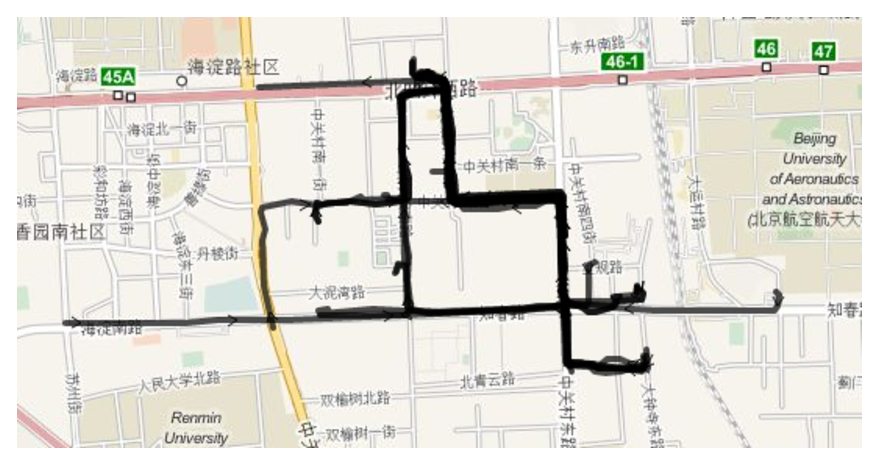
\includegraphics[width=6cm,height=4cm,keepaspectratio]{figs/new/Elbow_Cluster3.eps}
        \caption{Cluster 3(31 trajectories)}
    \end{subfigure}%
    \begin{subfigure}[t]{.5\textwidth}
        \centering
        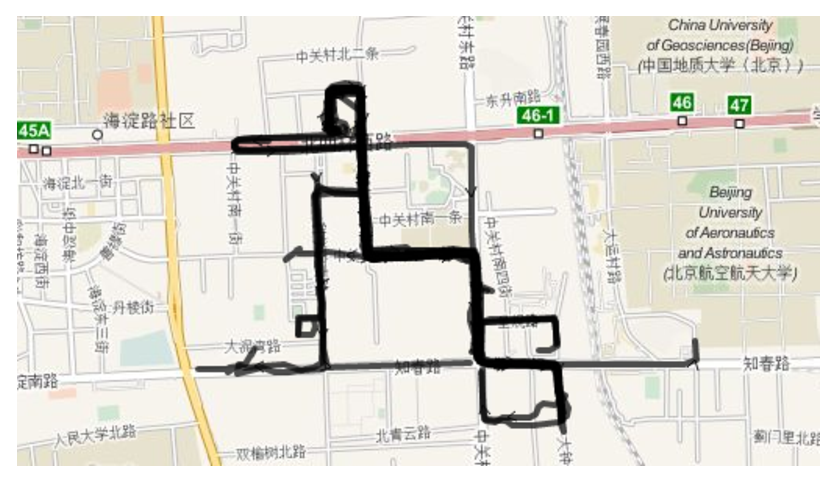
\includegraphics[width=6cm,height=4cm,keepaspectratio]{figs/new/Elbow_Cluster4.eps}
        \caption{Cluster 4(31 trajectories)}
    \end{subfigure}
    \caption{Visualizations of the top 4 clusters at Elbow Point}
    \label{fig:elbowVisual}
\end{figure*}

\begin{figure*}
    \centering
    \begin{subfigure}[t]{.5\textwidth}
        \centering
        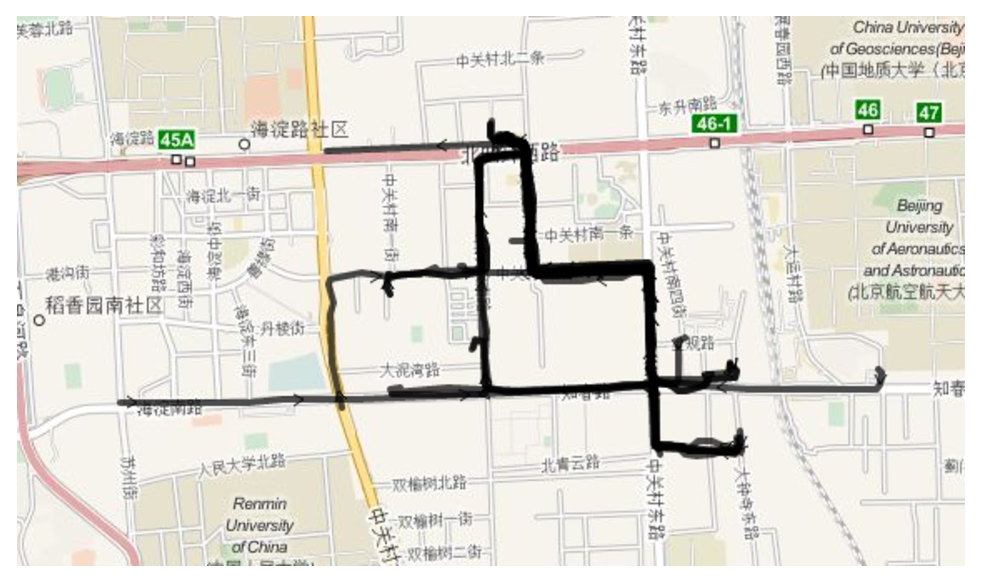
\includegraphics[width=6cm,height=4cm,keepaspectratio]{figs/new/Elbow5_Cluster1.eps}
        \caption{Cluster 1 ( 31 trajectories)}
    \end{subfigure}%
    ~ 
    \begin{subfigure}[t]{.5\textwidth}
        \centering
        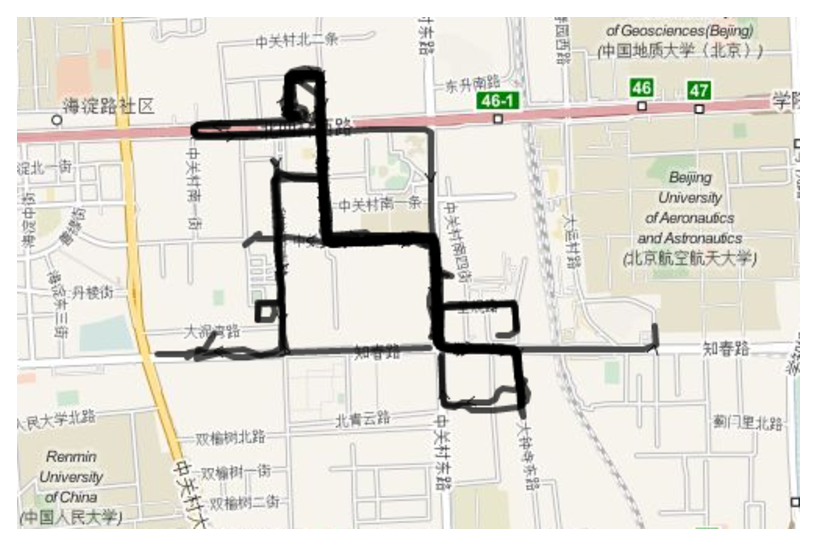
\includegraphics[width=6cm,height=4cm,keepaspectratio]{figs/new/Elbow5_Cluster2.eps}
        \caption{Cluster 2(31 trajectories)}
    \end{subfigure}
    
    \begin{subfigure}[t]{.5\textwidth}
        \centering
        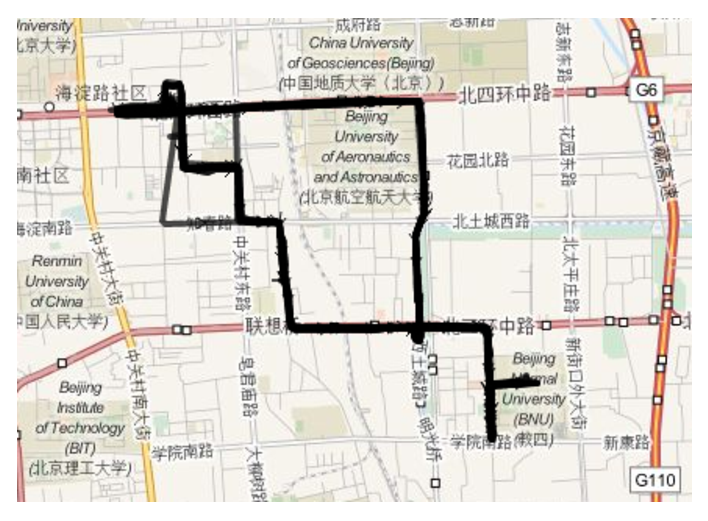
\includegraphics[width=6cm,height=4cm,keepaspectratio]{figs/new/Elbow5_Cluster3.eps}
        \caption{Cluster 3(24 trajectories)}
    \end{subfigure}%
    \begin{subfigure}[t]{.5\textwidth}
        \centering
        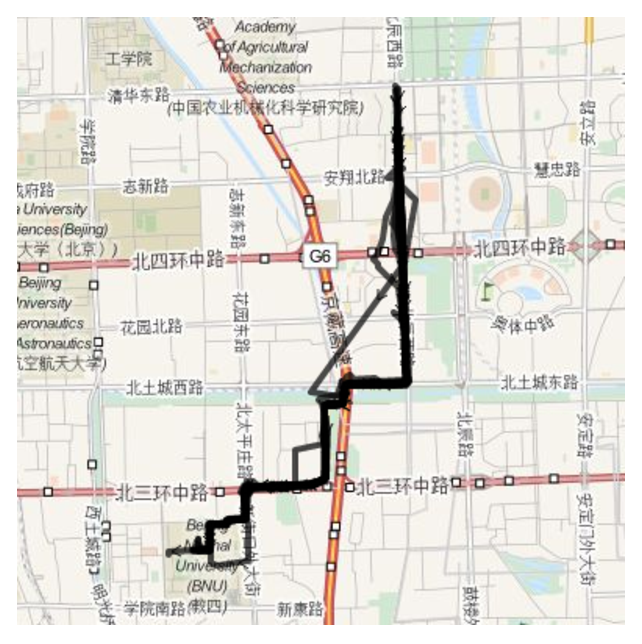
\includegraphics[width=6cm,height=4cm,keepaspectratio]{figs/new/Elbow5_Cluster4.eps}
        \caption{Cluster 4(20 trajectories)}
    \end{subfigure}
    \caption{Visualizations of the top 4 clusters at Elbow Point+5 point- Clusters not tight enough,need to go down the dendrogram further}
    \label{fig:elbow5visual}
\end{figure*}
Thus, we see that the elbow point does not get us anywhere close to the optimal number of clusters, but can help as a starting point for finding the optimal number. One insight that the elbow point gives is that the optimal point cant be before the elbow point, and hence we can prune the search space till the elbow point. 
The heuristic that we follow to obtain the optimal number of clusters is to traverse down the dendrogram , starting from the elbow point, and at any stage if we hit a cluster where the maximum pointwise distance between any pair of trajectories is less than $\delta$, we report it as a final cluster. 
\begin{figure*}
    \centering
    \begin{subfigure}[t]{.5\textwidth}
        \centering
        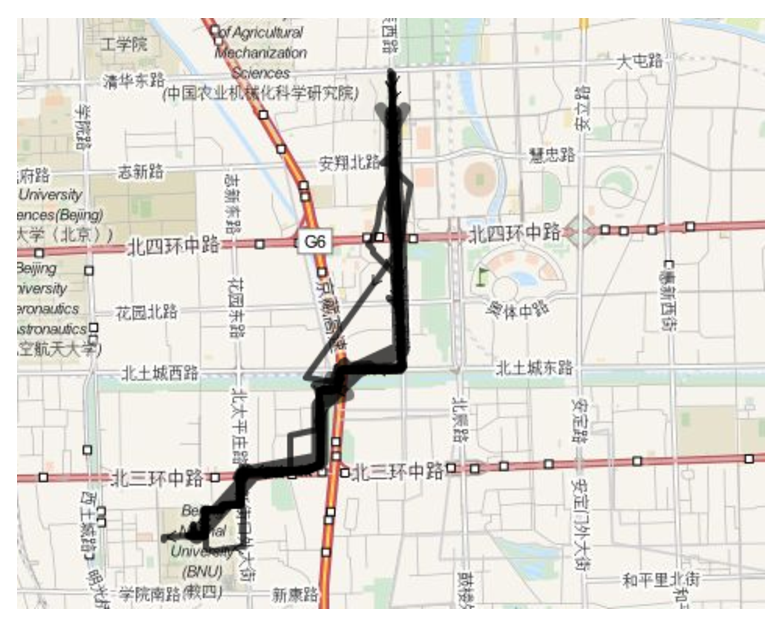
\includegraphics[width=6cm,height=4cm,keepaspectratio]{figs/new/FinalCluster1.eps}
        \caption{Cluster 1 ( 20 trajectories)}
    \end{subfigure}%
    ~ 
    \begin{subfigure}[t]{.5\textwidth}
        \centering
        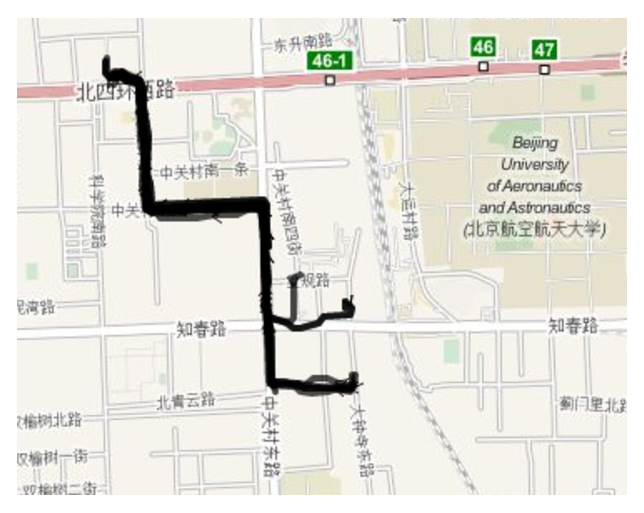
\includegraphics[width=6cm,height=4cm,keepaspectratio]{figs/new/FinalCluster2.eps}
        \caption{Cluster 2(15 trajectories)}
    \end{subfigure}
    
    \begin{subfigure}[t]{.5\textwidth}
        \centering
        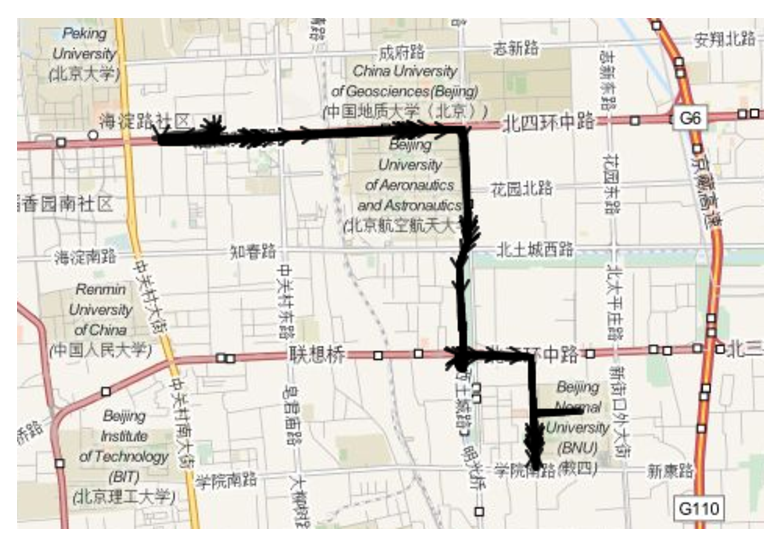
\includegraphics[width=6cm,height=4cm,keepaspectratio]{figs/new/FinalCluster3.eps}
        \caption{Cluster 3(11 trajectories)}
    \end{subfigure}%
    \begin{subfigure}[t]{.5\textwidth}
        \centering
        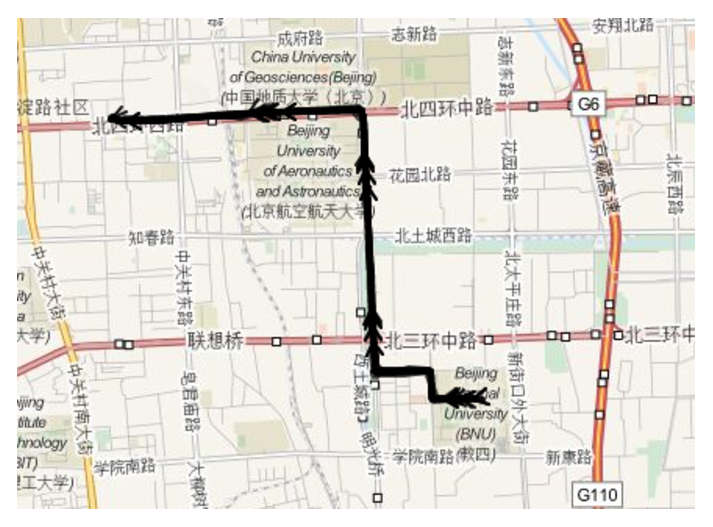
\includegraphics[width=6cm,height=4cm,keepaspectratio]{figs/new/FinalCluster4.eps}
        \caption{Cluster 4(9 trajectories)}
    \end{subfigure}
    \caption{Visualizations of the top 4 final optimal clusters}
    \label{fig:finalClusters}
\end{figure*}

Fig.\ref{fig:finalClusters} shows the visualizations of the top-4 clusters at the optimal level. 
\subsubsection{Variation with DBSCAN} 
In order to make an attempt at doing away with the heuristic, we tried another approach. In this approach we perform two stages of clustering followed by a DBSCAN based on the OD similarity measure we proposed. This method is described below : 
\begin{itemize}
\item In the first stage, we cluster the trajectories based on the Origin to origin distance. We run hierarchical clustering, and then plot the elbow curve for the SSW values and cluster it at the elbow point. 
\item In the next stage, we further cluster each cluster obtained from above based on the destination distances and performing hierarchical clustering individually on each of the clusters.
\item Once we have performed the origin and destination clusters, we now have trajectories clustered on their OD values. Now, on each of these individual clusters, we run DBSCAN based on the similarity proposed earlier. The values for minLns and epsilon are chosen using the heuristic mentioned in the paper .
\end{itemize}
By using this variant, we dont use the heuristic at any step, and are still successful in getting optimum results. The visualizations of the top 4 clusters by using this method is shown in Fig. \ref{fig:DBSCANRes}
\begin{figure*}
    \centering
    \begin{subfigure}[t]{.5\textwidth}
        \centering
        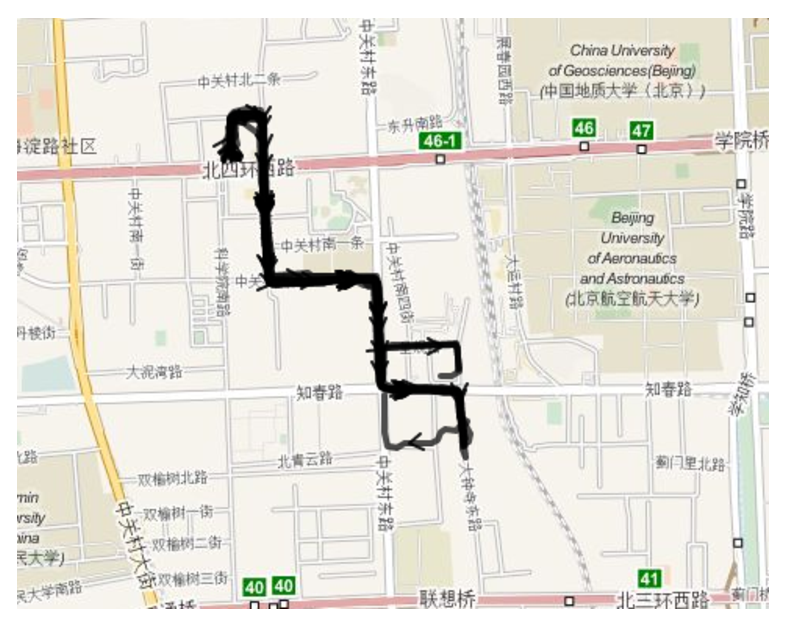
\includegraphics[width=6cm,height=4cm,keepaspectratio]{figs/new/DBSCAN1.eps}
        \caption{Cluster 1 ( 19 trajectories)}
    \end{subfigure}%
    ~ 
    \begin{subfigure}[t]{.5\textwidth}
        \centering
        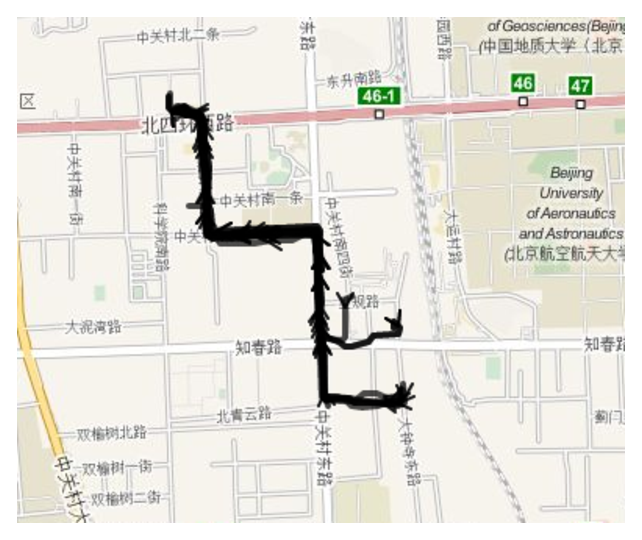
\includegraphics[width=6cm,height=4cm,keepaspectratio]{figs/new/DBSCAN2.eps}
        \caption{Cluster 2(16 trajectories)}
    \end{subfigure}
    
    \begin{subfigure}[t]{.5\textwidth}
        \centering
        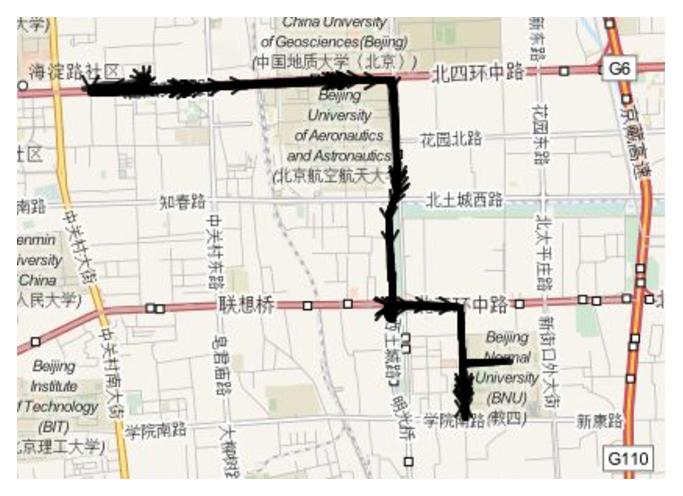
\includegraphics[width=6cm,height=4cm,keepaspectratio]{figs/new/DBSCAN3.eps}
        \caption{Cluster 3(11 trajectories)}
    \end{subfigure}%
    \begin{subfigure}[t]{.5\textwidth}
        \centering
        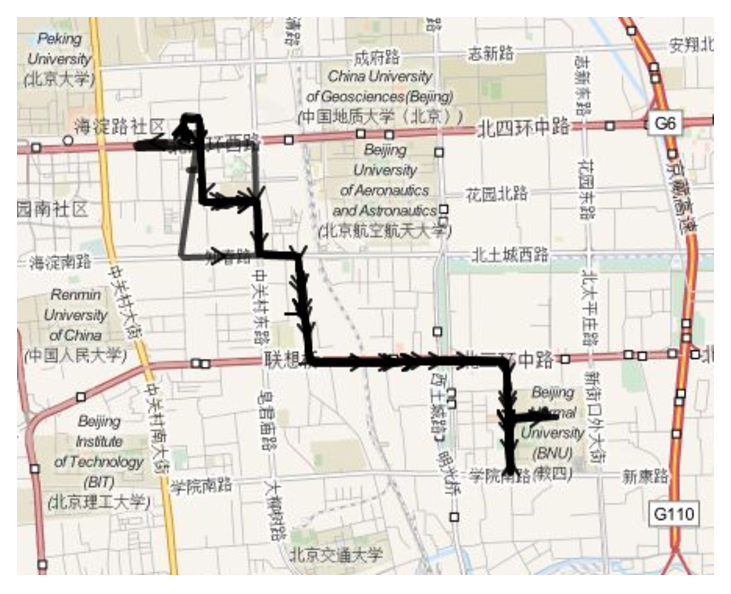
\includegraphics[width=6cm,height=4cm,keepaspectratio]{figs/new/DBSCAN4.eps}
        \caption{Cluster 4(9 trajectories)}
    \end{subfigure}
    \caption{Visualizations of the top 4 final optimal clusters using the DBSCAN variation}
    \label{fig:DBSCANRes}
\end{figure*}

\subsubsection{Comparisons with DTW}
The first comparison is made using Dynamic Time Warping as the similarity metric, and clustering based on that matrix.WE use the same framework as that proposed in our method, the only difference being that we plug in DTW similarity in place of our OD based similarity defined earlier. DTW is very close to our method considering the clustering effectiveness, but there are cases where it misses out trajectories that are a part of a meaningful trip summary. On the basis of computation time, our approach is way faster than DTW, because DTW heavily depends on the number of sample points. As the number of sample points increase, the time starts to blow up.

Problems with DTW
\begin{itemize}
\item
DTW is not a metric as it violates triangle inequality. This can lead to issues during clustering.Any distance metric d follows triangle inequality if, for any three points, x,y,and z: d(x, z) ≤ d(x, y) + d(y, z).     Figure \ref{fig:dtw_triangleineq} shows an example of the violation of triangle inequality using DTW similarity.
\begin{figure}
\centering     
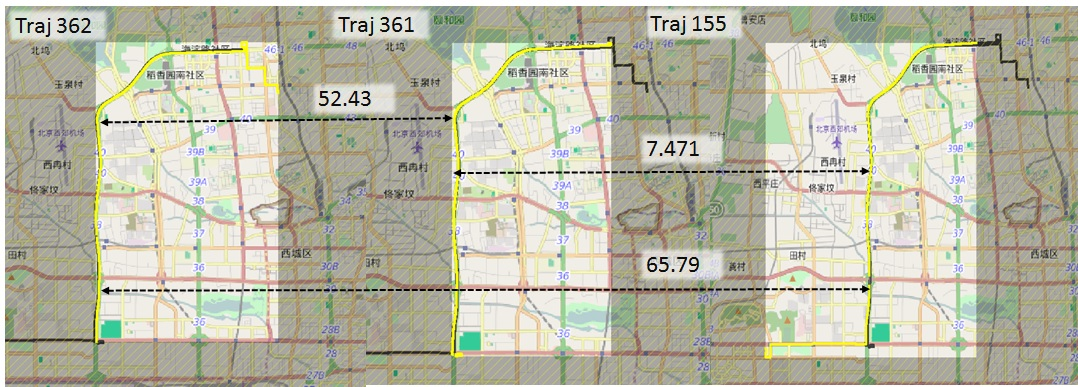
\includegraphics[scale=0.5]{figs/DTW_triangle_ineq.jpg}
\caption{Example of Triangle Inequality Violation using DTW }
\label{fig:dtw_triangleineq}  
\end{figure}

\item 
The biggest concern about DTW is the computation time. When the sample points are very large, it can get to as much as 400 times slower than the proposed approach. If the points are resampled and DTW similarity is computed, it would reduce to the same as pointwise Eucledian distance, and would still be computationally more expensive. Fig \ref{fig:time_dtw_od} shows the computation time differences over all the users for clustering using  DTW and OD similarity measures over all the users

\begin{figure}
\centering     
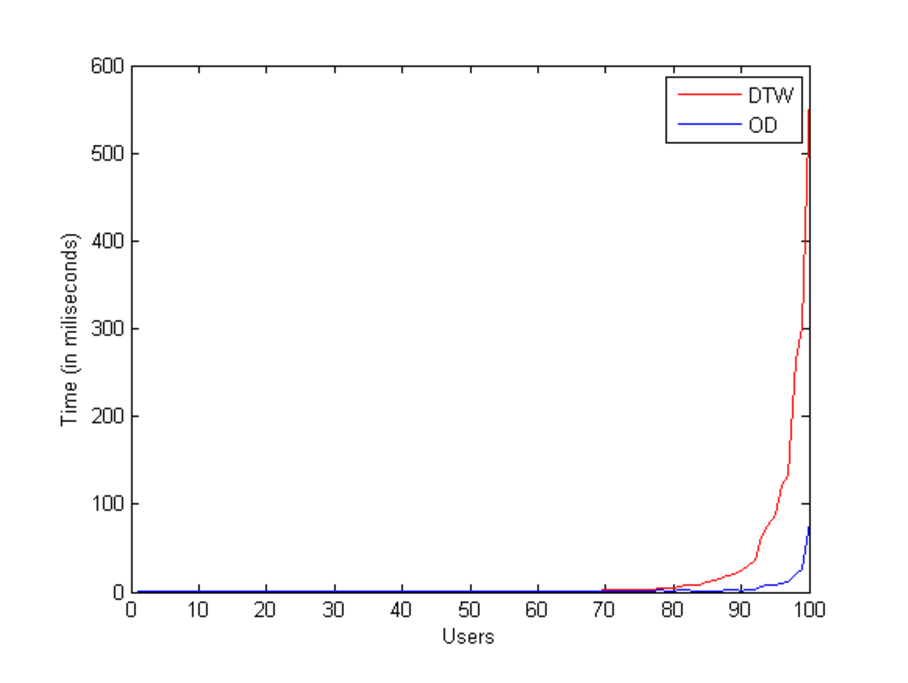
\includegraphics[scale=0.5]{figs/dtw_od_time.eps}
\caption{Computation time comparison of DTW and OD }
\label{fig:time_dtw_od}  
\end{figure}

\item
As we decrease the number of sample points, the effectiveness of both our proposed method and DTW go down. But the goodness of the clusters returned by DTW decreases more than that of the proposed method. We reduced the number of sample points in each of the trajectories to 90\%,95\%, and 97\% and plotted the silhouette coefficient values using DTW,LP and OD. 

\begin{figure*}
    \centering
    \begin{subfigure}[t]{.5\textwidth}
        \centering
        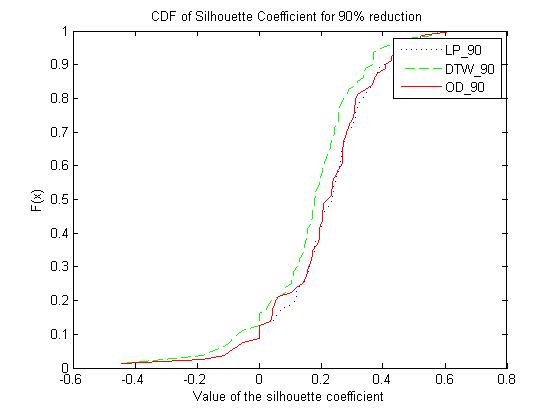
\includegraphics[scale=0.4]{figs/noise_90_cdf.jpg}
        \caption{CDF of the silhouette coefficient for 90\% reduction of sample points }
    \end{subfigure}%
	\begin{subfigure}[t]{.5\textwidth}
        \centering
        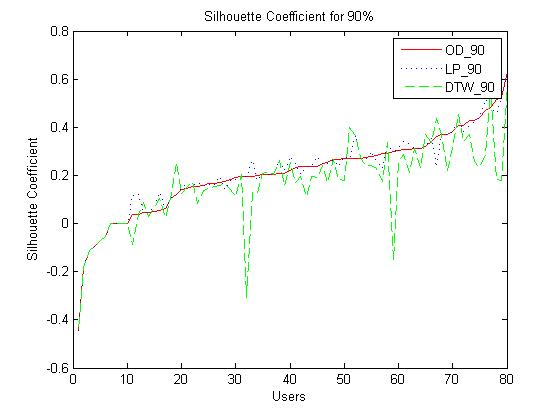
\includegraphics[scale=0.4]{figs/noise_90_sil.jpg}
        \caption{Plot of the silhouette coefficient for 90\% reduction of sample points}
    \end{subfigure}
     \caption{90\% reduction in sample points- Comparison of silhouette graphs}
    \label{fig:noise_90}    
\end{figure*}


\begin{figure*}
    \centering
    \begin{subfigure}[t]{.5\textwidth}
        \centering
        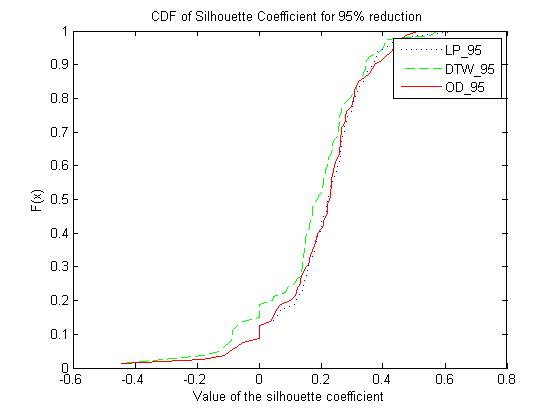
\includegraphics[scale=0.4]{figs/noise_95_cdf.jpg}
        \caption{CDF of the silhouette coefficient for 95\% reduction of sample points }
    \end{subfigure}%
	\begin{subfigure}[t]{.5\textwidth}
        \centering
        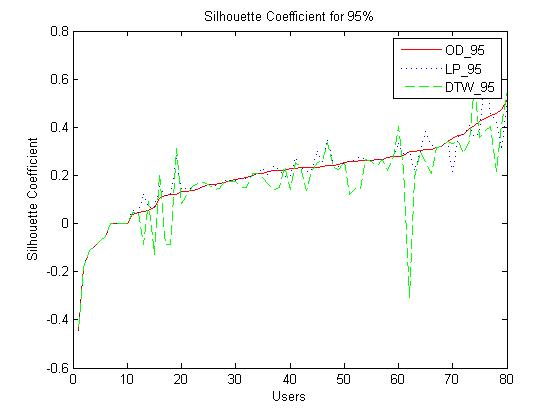
\includegraphics[scale=0.4]{figs/noise_95_sil.jpg}
        \caption{Plot of the silhouette coefficient for 95\% reduction of sample points}
    \end{subfigure}
    \caption{95\% reduction in sample points- Comparison of silhouette graphs}
    \label{fig:noise_95}       
\end{figure*}


\begin{figure*}
    \centering
    \begin{subfigure}[t]{.5\textwidth}
        \centering
        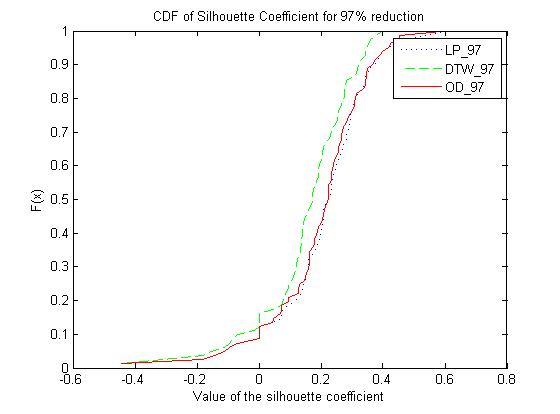
\includegraphics[scale=0.4]{figs/noise_97_cdf.jpg}
        \caption{CDF of the silhouette coefficient for 97\% reduction of sample points }
    \end{subfigure}%
	\begin{subfigure}[t]{.5\textwidth}
        \centering
        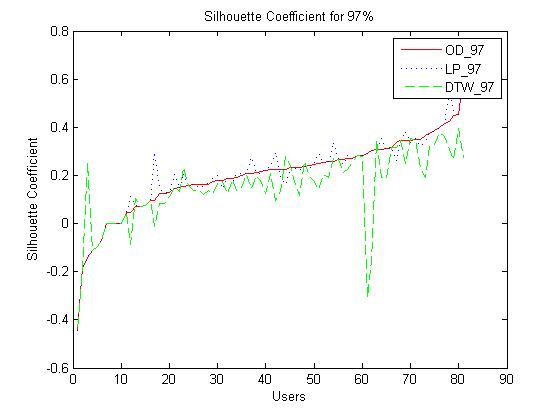
\includegraphics[scale=0.4]{figs/noise_97_sil.jpg}
        \caption{Plot of the silhouette coefficient for 97\% reduction of sample points}
    \end{subfigure}
    \caption{97\% reduction in sample points- Comparison of silhouette graphs}
    \label{fig:noise_97}       
\end{figure*}
\end{itemize}
\subsubsection{Comparison with SWARM}
The major problems with SWARM are as follows: 
\begin{itemize}
\item Does not report all the big clusters
\item Dependent a lot on the sample points. If we resample, it would be computationally more expensive than our approach.
\end{itemize}

We show that our method performs better than SWARM over all the users using the values of the Silhouette Coefficient of the resulting clusters in Fig \ref{fig:SWARM_OD}. We also show the CDF of the SSW of the resulting clusters of SWARM vs our method in Fig \ref{fig:SSW_SWARM}.
\begin{figure*}
    \centering
    \begin{subfigure}[t]{.5\textwidth}
        \centering
        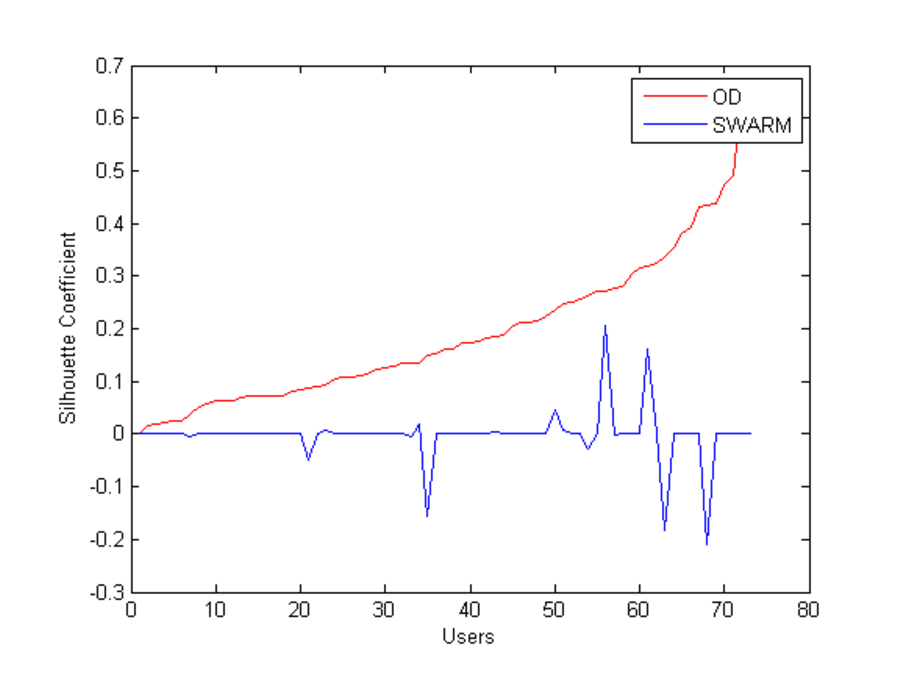
\includegraphics[scale=0.6]{figs/swarm_od_silcomparison.eps}
\caption{Silhouette Values of the resulting clusters for SWARM and OD- We perform significantly better over all users}
\label{fig:SWARM_OD}  
    \end{subfigure}%
	\begin{subfigure}[t]{.5\textwidth}
        \centering
        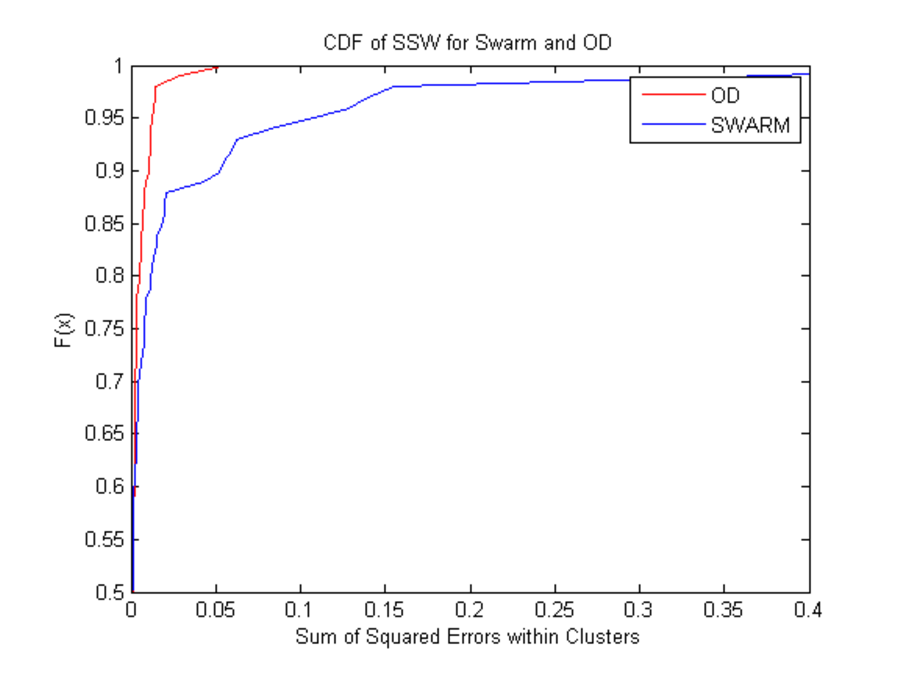
\includegraphics[scale=0.6]{figs/swarm_od_ssw.eps}
\caption{SSW Values of the resulting clusters for SWARM and OD- Our SSW error is lesser than SWARM over all users}
\label{fig:SSW_SWARM} 
    \end{subfigure}
    \caption{SWARM comparisons}
    \label{fig:swarm}       
\end{figure*}


\subsubsection{TraClus}
TraClus looks at the sub-trajectory level, and clusters trajectories on the basis of the similarities between those sub-trajectories. In the first phase, it partitions the trajectories into segments, and in the second phase, it clusters the partitions together using a DBSCAN-like technique.The problems with TrajClus are
\begin{itemize}

\item
The similarity measure between any two partitions is defined as a weighted sum of the perpendicular distance, parallel distance and the angular distance between the partitions. Here, three quantities with different units are being merged together, so when two partitions are similar, it is difficult to say which distance contributed to the similarity. Also, this creates a problem in arriving at the neighbourhood parameters. 

\item
 There are two parameters used in this algorithm, \textit{epsilon} and \textit{minLns}. \textit{epsilon} defines the neighourhood reach of each of the partition, and minLns is the minimum number of Partitions required in the neighbourhood for it to be considered as a cluster. The authors suggest a simulated annealing technique to arrive at the value of epsilon , and from that value, further calculate the value of minLns. But, because the algorithm is highly associative, nearly all the partitions end up in one cluster, thus not identifying the correct movement summaries. 
   
   
\begin{figure*}
    \centering
    \begin{subfigure}[t]{.5\textwidth}
        \centering
        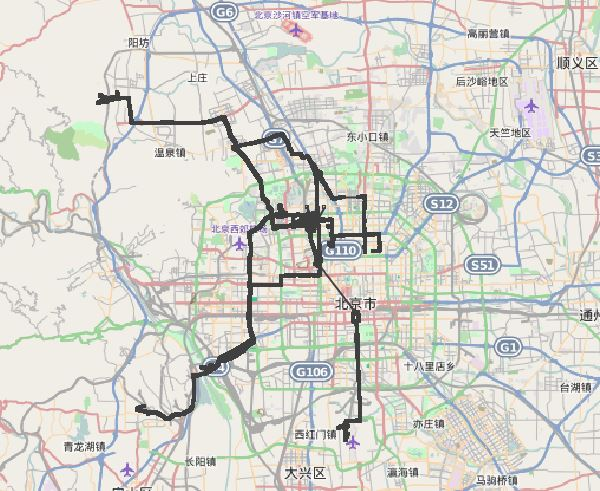
\includegraphics[scale=0.4]{figs/TrajClus_full.jpg}
        \caption{All the trajectories of an example user }
\label{fig:TrajClus_full}  
    \end{subfigure}%
	\begin{subfigure}[t]{.5\textwidth}
        \centering
        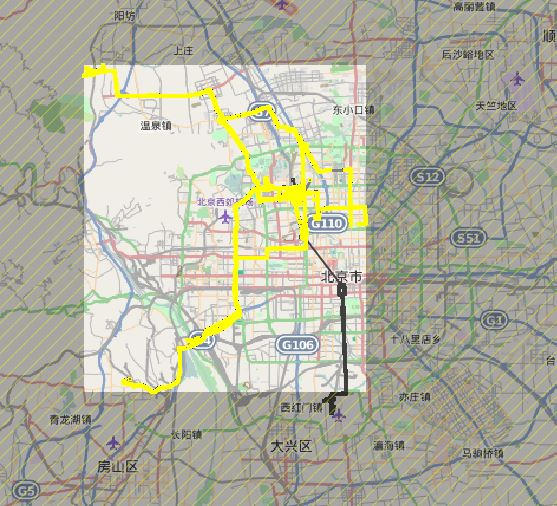
\includegraphics[scale=0.4]{figs/TrajClus_cluster.jpg}
\caption{Cluster reported by TraClus}
\label{fig:TrajClus_cluster}  
    \end{subfigure}
    \caption{TraClus Final cluster reported}
    \label{fig:traclus}       
\end{figure*}


\item

TrajClus does not give enough weightage to the direction of the line segment. In cases like animal movement or hurricane movement, this makes sense, because there wont be many cases of trajectories in different directions in a flock or cluster. But when it comes to human movement pattern, directions play a very important role in determining the movement summaries of a person. TrajClus overlooks it and clusters two trajectories in different directions in the same cluster.

\begin{figure}
\centering     
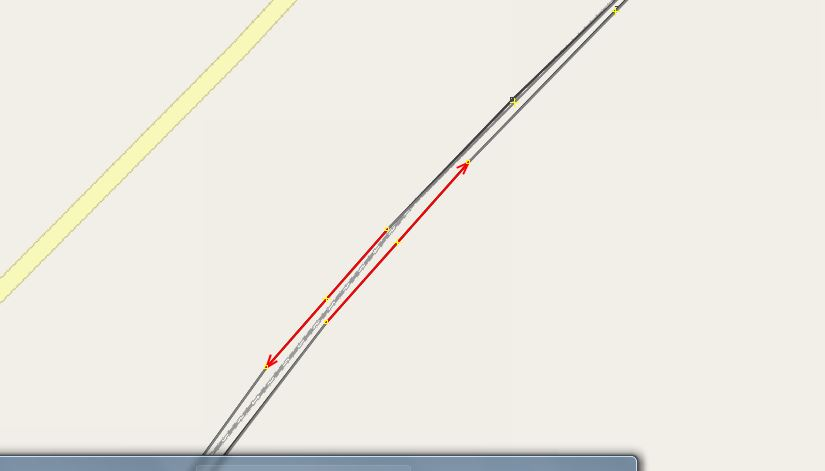
\includegraphics[scale=0.3]{figs/direction.jpg}
\caption{Trajectories with different directions clustered together by TrajClus}
\label{fig:TrajClus_direction}  
\end{figure}

\end{itemize}
\subsubsection{Next Location Prediction}
Another way to test the summarization of the movement patterns is to test a query trajectory and plot its predicted next location/destination as predicted by all the methods.

The next location prediction is done by the following algorithm:
\paragraph{Explanation of the algo}
For any query trajectory, resample, and compute similarity with the median trajectories of all summary clusters. Report the one with the maximum similarity. 


Let $g(i)$ be the probability of the summary $i$. Given an input traj $t_{\operatorname{in}}$, compute the distance (in meters or so) $d(i,t_{\operatorname{in}})$ between summary $i$ and $t_{\operatorname{in}}$. Now the probability that this sub-trajectory lies within summary $i$ is given by
\begin{eqnarray}
p(i,t_{\operatorname{in}}) = \frac{1}{\sqrt{2 \pi} \sigma_{t}} \mathrm{e}^{-0.5 \left( \frac{d(i,t_{\operatorname{in}})}{\sigma_{t}} \right)}
\end{eqnarray}
Here we assume that the input trajectory is a noisy input from GPS samples. $\sigma_{t}$ is the standard deviation of the sub-trajectory distance. For now take, $\sigma_{t} = \sigma_{p}$, where $\sigma_{p}$ is the standard deviation of the GPS sampling a location (value is 15.61, which is the 95-th percentile of GPS considering 30 m error). It should ideally be standard deviation introduced when we compute distance between 100 points of a path

For each of the methods compared, we plot the CDF of the error of the predicted destination for the Top-3 Closest clusters to each of the query trajectories. Each of the graphs contain 4 plots, each one varying the number of sample points given to the query trajectory. We have plotted the errors for query trajectories with 10\%, 25 \%, 50\% and 90\% of the sample points. 

\begin{figure*}
    \centering
    \begin{subfigure}[t]{.5\textwidth}
        \centering
        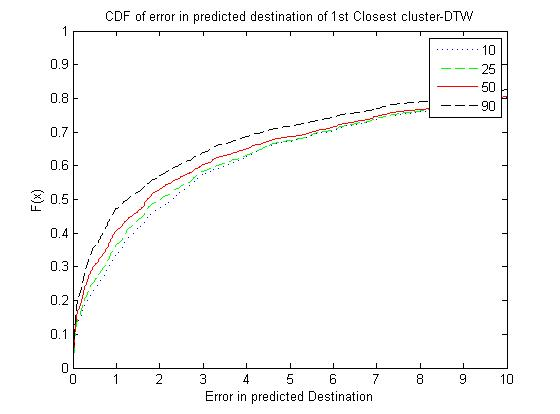
\includegraphics[scale=0.4]{figs/dtw_top.jpg}
        \caption{CDF of error in predicted destination for 1st closest cluster using DTW}
    \end{subfigure}%
	\begin{subfigure}[t]{.5\textwidth}
        \centering
        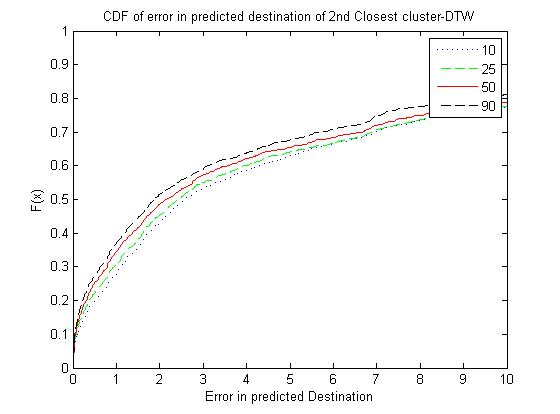
\includegraphics[scale=0.4]{figs/dtw_top2.jpg}
        \caption{CDF of error in predicted destination for 2nd closest cluster using DTW}
    \end{subfigure}
    \begin{subfigure}[t]{.5\textwidth}
        \centering
        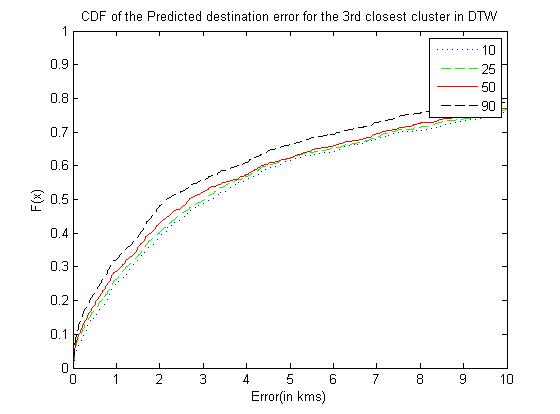
\includegraphics[scale=0.4]{figs/dtw_top3.jpg}
        \caption{CDF of error in predicted destination for 3rd closest cluster using DTW}
    \end{subfigure}
    \caption{CDF of the error in predicted destinations for the top 1,2,3 closest clusters for \emph{DTW}}
    \label{fig:nextloc_DTW}       
\end{figure*}

\begin{figure*}
    \centering
    \begin{subfigure}[t]{.5\textwidth}
        \centering
        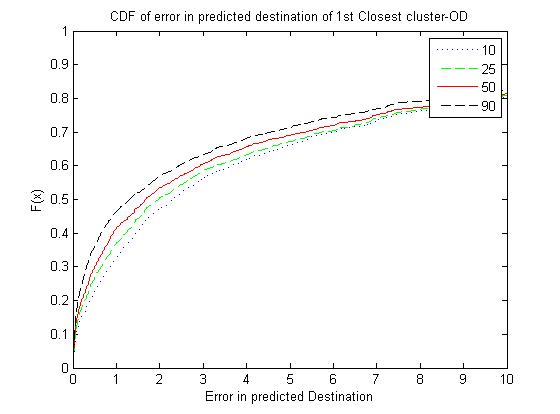
\includegraphics[scale=0.4]{figs/od_top.jpg}
        \caption{CDF of error in predicted destination for 1st closest cluster using OD}
    \end{subfigure}%
	\begin{subfigure}[t]{.5\textwidth}
        \centering
        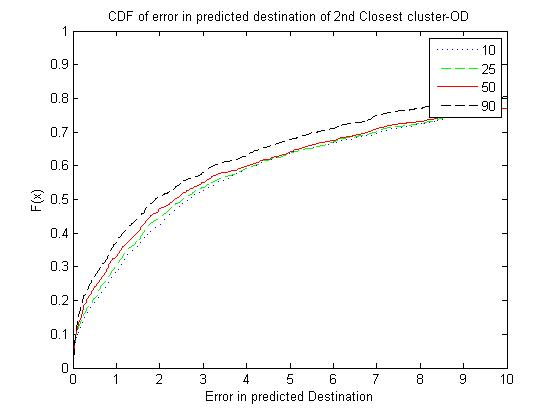
\includegraphics[scale=0.4]{figs/od_top2.jpg}
        \caption{CDF of error in predicted destination for 2nd closest cluster using OD}
    \end{subfigure}
    \begin{subfigure}[t]{.5\textwidth}
        \centering
        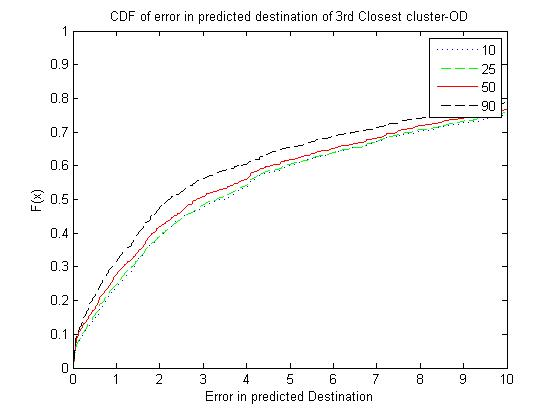
\includegraphics[scale=0.4]{figs/od_top3.jpg}
        \caption{CDF of error in predicted destination for 3rd closest cluster using OD}
    \end{subfigure}
    \caption{CDF of the error in predicted destinations for the top 1,2,3 closest clusters for \emph{OD}}
    \label{fig:nextloc_OD}       
\end{figure*}

\begin{figure*}
    \centering
    \begin{subfigure}[t]{.5\textwidth}
        \centering
        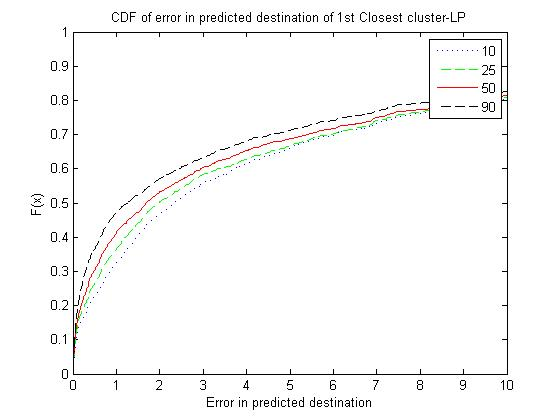
\includegraphics[scale=0.4]{figs/lp_top.jpg}
        \caption{CDF of error in predicted destination for 1st closest cluster using LP}
    \end{subfigure}%
	\begin{subfigure}[t]{.5\textwidth}
        \centering
        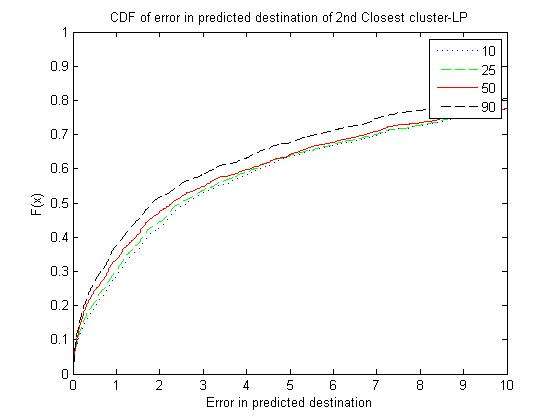
\includegraphics[scale=0.4]{figs/lp_top2.jpg}
        \caption{CDF of error in predicted destination for 2nd closest cluster using LP}
    \end{subfigure}
   \caption{CDF of the error in predicted destinations for the top 1,2 closest clusters for \emph{LP}}
    \label{fig:nextloc_LP}       
\end{figure*}

\begin{figure*}
    \centering
    \begin{subfigure}[t]{.5\textwidth}
        \centering
        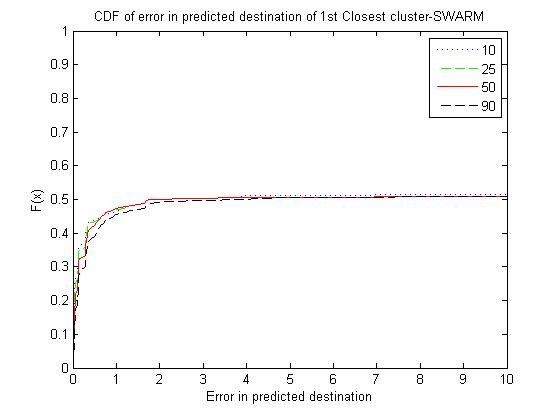
\includegraphics[scale=0.4]{figs/swarm_top.jpg}
        \caption{CDF of error in predicted destination for 1st closest cluster using SWARM}
    \end{subfigure}%
	\begin{subfigure}[t]{.5\textwidth}
        \centering
        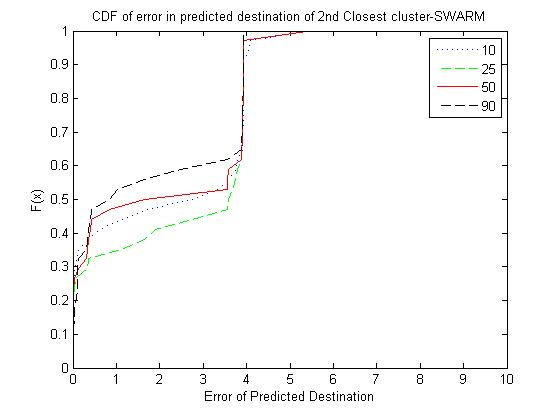
\includegraphics[scale=0.4]{figs/swarm_top2.jpg}
        \caption{CDF of error in predicted destination for 2nd closest cluster using SWARM}
    \end{subfigure}
   \caption{CDF of the error in predicted destinations for the top 1,2 closest clusters for \emph{SWARM}}
    \label{fig:nextloc_SWARM}       
\end{figure*}


Some of the observations from the next location prediction results are as follows:\\
Our Approach and LP predict the destination of \emph{82\%} of the trajectories with less than 10km error for closest cluster. 
DTW also is very close with prediction \emph{80\%} of the trajectories, but SWARM fares very badly with just \emph{5\%} of the trajectories' destination predicted. SWARM cannot detect the third closest cluster for any of the input trajectories. 



%Extra Graphs --->
%\begin{figure}
%\centering     
%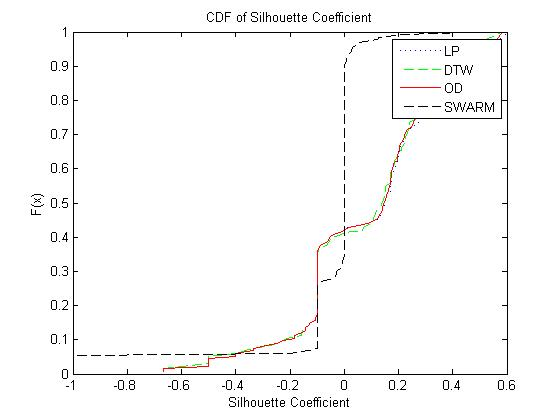
\includegraphics[scale=0.3]{figs/testing_sil.jpg}
%\caption{Comparison of silhouette coefficients for different schemes: OD- and LP-based clustering outperform existing mechanism. }
%\label{fig:sil_cdf}  
%\end{figure}
%
%The CDF plot shows that  DTW is very similar to our approach in terms of clustering effectiveness, but SWARM does a very poor job. 
%
%\subsubsection{Average Trajectories Per Cluster}
%Number of clusters with large number of trajectories in it is better (Figure~\ref{fig:avg_cdf} and ~\ref{fig:avgtop_cdf}). 
%
%\begin{figure}[H]
%\centering     
%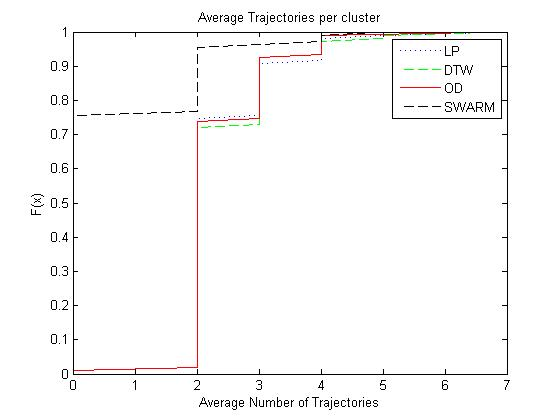
\includegraphics[scale=0.3]{figs/avg.jpg}
%\caption{CDF of Average trajectories per cluster for LP-DTW-OD}
%\label{fig:avg_cdf}  
%\end{figure} 
%
%\begin{figure}[H]
%\centering     
%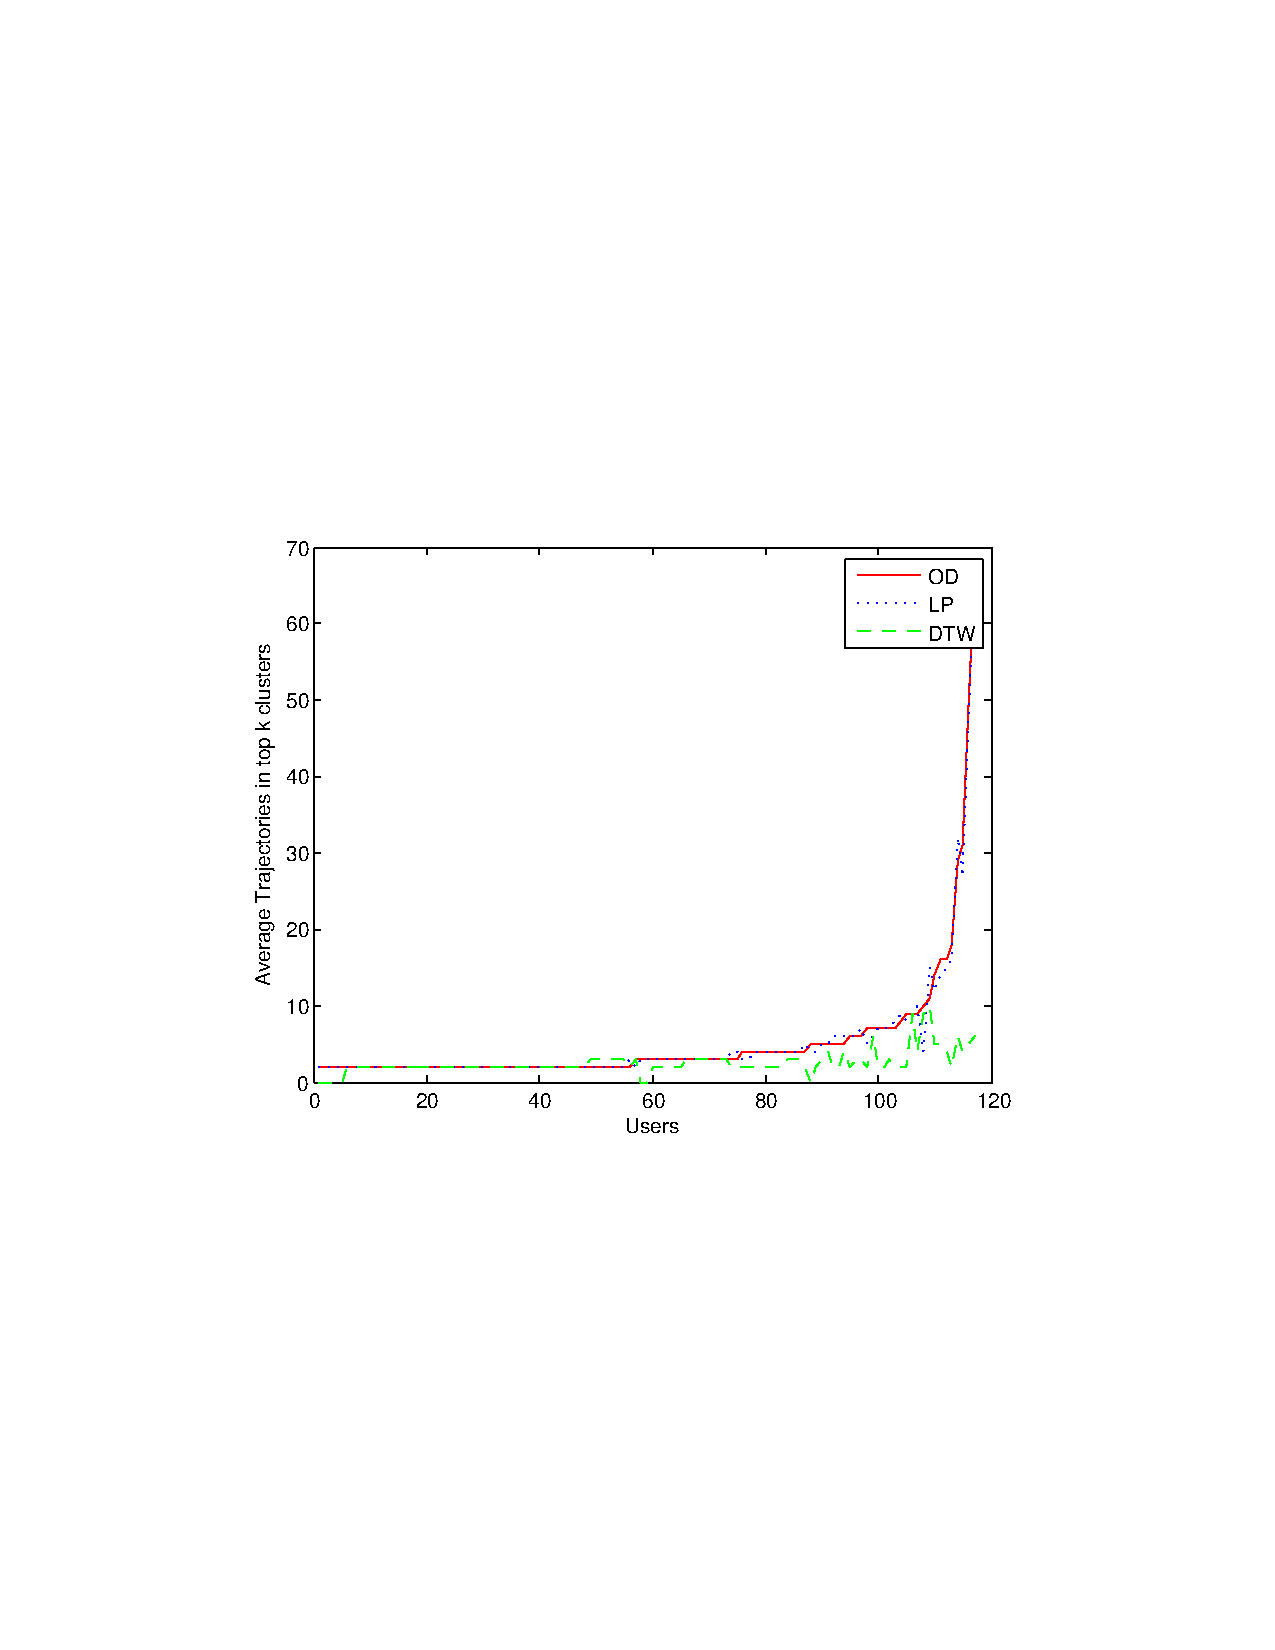
\includegraphics[scale=0.3]{figs/avgtop.jpg}
%\caption{CDF of Average trajectories per top-k clusters for LP-DTW-OD}
%\label{fig:avgtop_cdf}  
%\end{figure} 
%
%\subsection{Computation Time}
%
%\begin{figure}[H]
%\centering     
%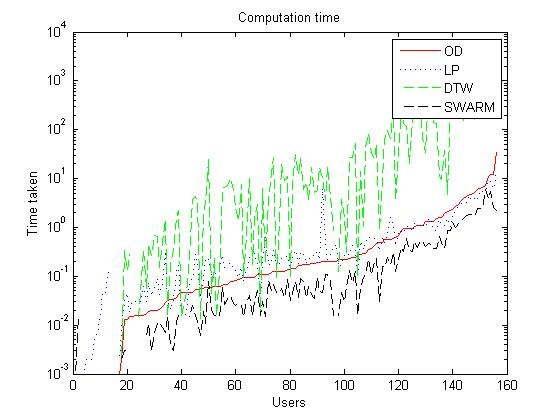
\includegraphics[scale=0.3]{figs/time_log.jpg}
%\caption{Computation time  for LP-DTW-OD}
%\label{fig:time_cdf}  
%\end{figure} 
%
%
%



%\subsubsection{Visualization at various granularity }
%%\rednote {Remove later if needed}
%
%\begin{figure*}
%\centering   
%\includegraphics[scale=0.6]{figs/demo.jpg}
%\caption{Visualization at various zoom levels}
%\label{fig:demo}  
%\end{figure*}
%
%\subsubsection{Case Study: Reported Final Clusters from each method}
%
%We take up a sample case, and show the snapshots of the final clusters as reported by all the different methods. DTW and OD have similar final clusters whereas SWARM reports only final clusters. 
%
%
%\begin{figure}
%\centering     
%\includegraphics[scale=0.4]{figs/snapshot_swarm.jpg}
%\caption{Snapshot of clusters reported by SWARM }
%\label{fig:casestudy_swarm}  
%\end{figure} 
%
% 
%\begin{figure}
%\centering     
%\includegraphics[scale=0.4]{figs/snapshot_od.jpg}
%\caption{Snapshot of clusters reported by OD}
%\label{fig:casestudy_od}  
%\end{figure} 
%
%\begin{figure}
%\centering     
%\includegraphics[scale=0.4]{figs/snapshot_dtw.jpg}
%\caption{Snapshot of clusters reported by DTW}
%\label{fig:casestudy_dtw}  
%\end{figure} 
%
%\iffalse
%The table below shows the statistics of the top k clusters and the number of trajectories 
%
%\begin{table*}
%	\centering
%		\begin{tabular}{|c|c|c|c|c|} 
%			\hline
%			Method&DTW&SWARM&TrajClus&OD\\
%			\hline
%			Number of Clusters Reported&1&4&0&18\\
%			Number of trajectories in top 3 Clusters & 5&36,15,13&0&38,37,29\\
%			\hline
%		\end{tabular}
%	\caption{Comparison for case study}
%	\label{tab:case_study}
%\end{table*}
%\fi


\section{Conclusion and Future Work}

From a raw input of GPS traces, the final clusters of the \emph{movement summary} have been reported. This included preprocessing, defining a similarity measure, clustering the trajectories, and coming up with a heuristic to determine the optimal number of clusters. 
In future, the following activities will be taken up - comparisons for trajectory clustering, devising a better heuristic to find the optimal number of clusters, trajectory summarization, an efficient way of storing the clusters, and applications of \emph{mobility summary}.

%\section{Conclusion}

%% ADd the below at right places


\balance
\bibliographystyle{abbrv}
\bibliography{refs}
\end{document}
